\documentclass[a4paper]{article}

% CJK support: prefer ctex, fallback to XeTeX native line breaking
\IfFileExists{ctex.sty}{
  \usepackage[fontset=fandol]{ctex}
}{
  % Fallback for minimal TeX installs (e.g. MacTeX Basic, TeX Live scheme-basic)
  % without ctex/xeCJK. Uses XeTeX's built-in CJK line breaking.
  \usepackage{fontspec}
  \XeTeXlinebreaklocale "zh"
  \XeTeXlinebreakskip = 0pt plus 1pt
  \IfFontExistsTF{Songti SC}{\setmainfont{Songti SC}}{%
    \IfFontExistsTF{Noto Serif CJK SC}{\setmainfont{Noto Serif CJK SC}}{}%
  }
  \IfFontExistsTF{Heiti SC}{\setsansfont{Heiti SC}}{%
    \IfFontExistsTF{Noto Sans CJK SC}{\setsansfont{Noto Sans CJK SC}}{}%
  }
}

% Basic packages
\usepackage{amsmath, amssymb}
\usepackage{graphicx}
\usepackage[margin=2.5cm]{geometry}
\emergencystretch=3em
\usepackage[most]{tcolorbox}
\usepackage{etoolbox}
\usepackage{listings}
\usepackage{hyperref}
\usepackage{booktabs}
\usepackage{array}
\usepackage{subcaption}
\usepackage{float}
\usepackage{tikz}
\IfFileExists{pgfplots.sty}{
    \usepackage{pgfplots}
    \pgfplotsset{compat=1.18}
}{}

% ===== Highlight boxes =====
\newtcolorbox{knowledgebox}[1]{
    enhanced, colback=blue!5!white, colframe=blue!75!black, colbacktitle=blue!75!black,
    coltitle=white, fonttitle=\bfseries, title={#1}, attach boxed title to top left={yshift=-2mm, xshift=2mm},
    boxrule=1pt, sharp corners
}

\newtcolorbox{importantbox}[1]{
    enhanced, colback=yellow!10!white, colframe=yellow!80!black, colbacktitle=yellow!80!black,
    coltitle=black, fonttitle=\bfseries, title={#1}, sharp corners
}

\newtcolorbox{warningbox}[1]{
    enhanced, colback=red!5!white, colframe=red!75!black, colbacktitle=red!75!black,
    coltitle=white, fonttitle=\bfseries, title={#1}, sharp corners
}

\newtcolorbox{practicebox}[1]{
    enhanced, colback=black!3!white, colframe=black!75, colbacktitle=black!75,
    coltitle=white, fonttitle=\bfseries, title={#1}, sharp corners
}

% ===== Code listings =====
\lstset{
    basicstyle=\ttfamily\small,
    keywordstyle=\color{blue},
    stringstyle=\color{red!60!black},
    commentstyle=\color{green!60!black},
    breaklines=true,
    frame=single,
    numbers=left,
    numberstyle=\tiny\color{gray},
    captionpos=b,
    extendedchars=false
}

% ===== Figure provenance and unit macros =====
% \vtag goes inside \caption{...}; \srcnote{MM:SS--MM:SS} follows the figure environment.
\newcommand{\vtag}{\protect\footnotemark}
\newcommand{\srcnote}[1]{\footnotetext{视频画面时间区间：#1。若为裁剪图，时间区间仍对应原视频画面。}}
% Units work in text and math mode; never hand-write $^\circ$ or \AA inside \mathrm.
\newcommand{\degC}{\ensuremath{^{\circ}\mathrm{C}}}
\newcommand{\um}{\ensuremath{\mu\mathrm{m}}}
\newcommand{\nm}{\ensuremath{\mathrm{nm}}}
\newcommand{\angstrom}{\ensuremath{\text{\AA}}}

% ===== Front-page metadata =====
% Fill these in when generating notes.
\newcommand{\notetitle}{旋转}
\newcommand{\notesubtitle}{GAMES001 图形学中的数学 · 第 4 集：旋转矩阵、欧拉角、轴角、四元数、插值与角速度}
\newcommand{\noteauthors}{根据 GAMES-Webinar 直播录像整理（阮良旺 主讲）}
\newcommand{\notedate}{2024年3月25日（直播）}
\newcommand{\videochannel}{GAMES-Webinar（哔哩哔哩）}
\newcommand{\videopublishdate}{2024年3月6日（合集）}
\newcommand{\videoduration}{1小时55分49秒}
\newcommand{\videourl}{https://www.bilibili.com/video/BV1MF4m1V7e3/?p=4}
\newcommand{\videocoverpath}{cover.jpg}

\begin{document}

% ===== Title page =====
\begin{titlepage}
\centering
{\Large 课程笔记\par}
\vspace{1.2cm}
{\huge\bfseries \notetitle\par}
\ifdefempty{\notesubtitle}{}{
\vspace{0.3cm}
{\large \notesubtitle\par}
}
\vspace{0.5cm}
{\large \noteauthors\par}
\vspace{0.3cm}
{\large \notedate\par}
\vspace{1.0cm}

\ifdefempty{\videocoverpath}{
{\small 请在生成笔记时填入视频封面图的本地路径。\par}
}{
\includegraphics[width=0.82\textwidth,height=0.40\textheight,keepaspectratio]{\videocoverpath}\par
}

\vfill
\begin{tcolorbox}[width=0.9\textwidth, colback=black!2!white, colframe=black!60, sharp corners]
\textbf{视频作者/频道}：\videochannel\par
\textbf{发布日期}：\videopublishdate\par
\textbf{视频时长}：\videoduration\par
\textbf{视频链接}：
\ifdefempty{\videourl}{
未填写
}{
\href{\videourl}{\nolinkurl{\videourl}}
}
\end{tcolorbox}
\end{titlepage}

\tableofcontents
\newpage

%% --- 正文内容开始 --- %%

\section{这一讲要解决什么问题}

第四讲开始换了主讲人。阮良旺介绍说，前两讲线性代数基础和第三讲计算几何由倪星宇讲授，从“旋转变换”开始的四讲由他来讲。本讲的主题是\textbf{旋转}：旋转矩阵从哪里来、有什么性质，三维旋转在计算机里有哪些表示方法，各种表示怎么插值，以及角速度和旋转是什么关系。

讲者先用一张简单的图回顾了旋转：把一头奶牛绕 $x$ 轴顺时针旋转 $30^\circ$，点 $\mathbf p$ 变为 $\mathbf p'=\mathrm R\mathbf p$，其中
\[
\begin{pmatrix}x'\\y'\\z'\end{pmatrix}=
\begin{pmatrix}1&0&0\\0&\cos30^\circ&\sin30^\circ\\0&-\sin30^\circ&\cos30^\circ\end{pmatrix}
\begin{pmatrix}x\\y\\z\end{pmatrix}.
\]
这种“绕固定轴转一个角度”的旋转在前面的课程里已经介绍过。

\noindent\begin{minipage}{\textwidth}
\begin{figure}[H]
\centering
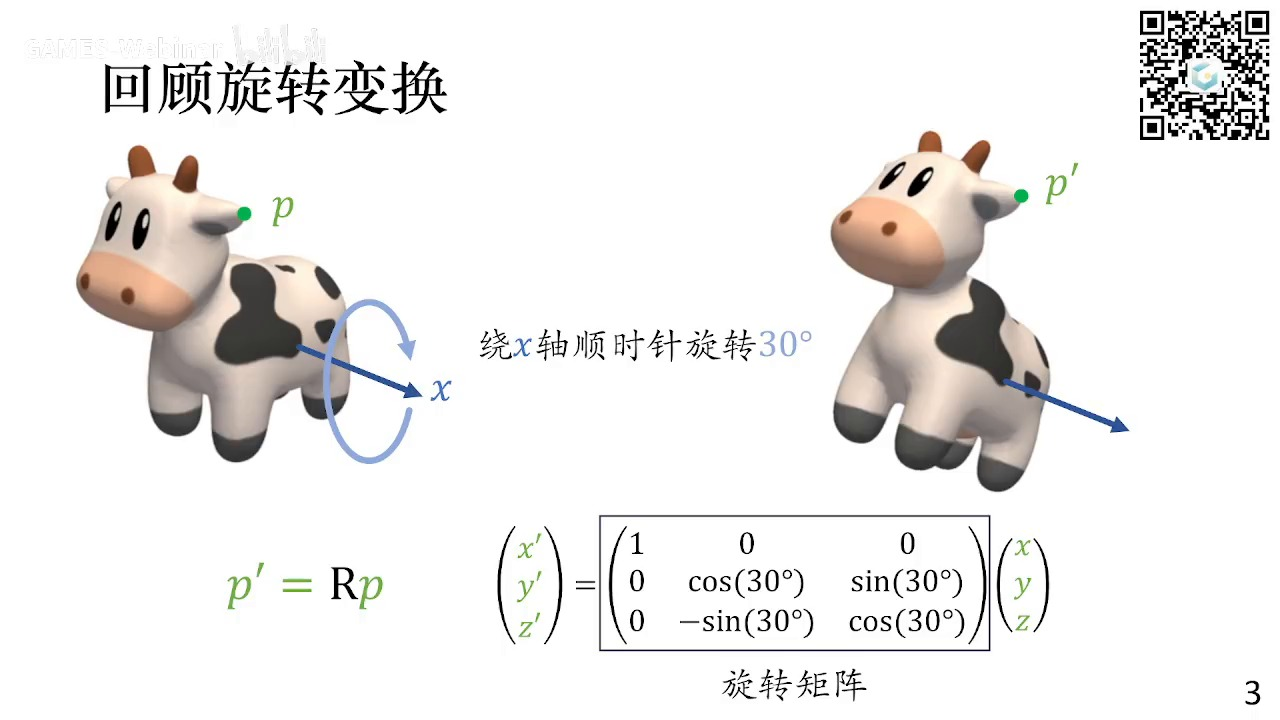
\includegraphics[width=0.92\textwidth]{figures/fig_01_review_rotation.jpg}
\caption{回顾旋转变换：奶牛绕 $x$ 轴顺时针旋转 $30^\circ$，$\mathbf p'=\mathrm R\mathbf p$\vtag}
\end{figure}
\srcnote{00:01:45--00:02:00}
\end{minipage}


接着他播放了一段 NASA 在空间站里拍摄的视频：一个 T 字形扳手在失重环境中被拨动，它的运动和绕固定轴的简单旋转有本质区别，非常复杂，\emph{没有定轴}。如何描述和分析这样的旋转，就是本讲要讨论的主要问题。

\noindent\begin{minipage}{\textwidth}
\begin{figure}[H]
\centering
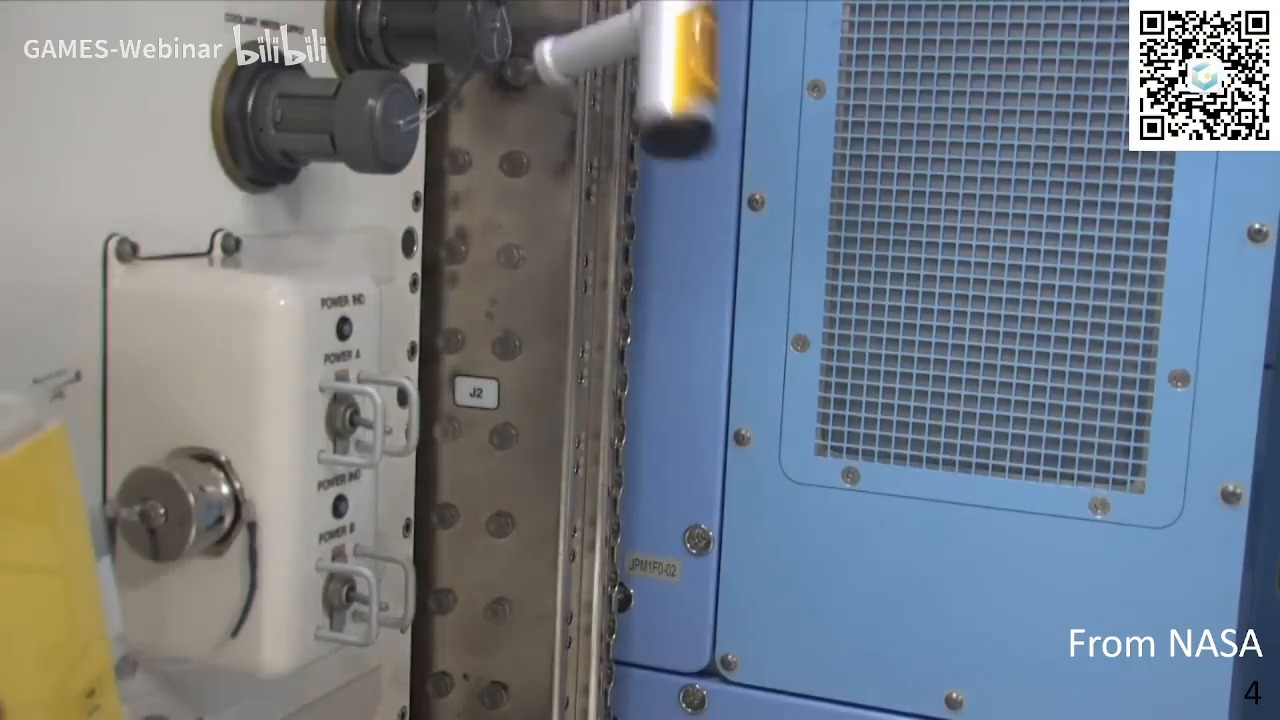
\includegraphics[width=0.92\textwidth]{figures/fig_02_nasa_video.jpg}
\caption{NASA 空间站视频：T 字形扳手在失重环境中的旋转没有固定的转轴\vtag}
\end{figure}
\srcnote{00:02:45--00:03:00}
\end{minipage}


\begin{importantbox}{本讲的主线}
本讲的逻辑是：先从“刚体运动保持距离”推出旋转矩阵必须是行列式为 $+1$ 的正交矩阵，即特殊正交群 $SO(3)$；再说明三维旋转只有 3 个自由度，构成 9 维空间中的 3 维流形，所以“旋转表示”本质上是\textbf{流形的参数化}；然后依次介绍欧拉角、轴角（旋转向量）和四元数三种参数化，比较它们的插值方法和优缺点；最后讨论神经网络适合的旋转表示，以及角速度与旋转矩阵、四元数导数的关系。
\end{importantbox}

\section{旋转矩阵与特殊正交群}

\subsection{从“保持距离”推出正交矩阵}

考虑一般的三维线性变换 $\mathbf p'=\mathrm A\mathbf p$，$\mathrm A\in\mathbb R^{3\times3}$。旋转是刚性的，物体上任意两点之间的距离在旋转前后不变：
\[
\mathbf p'-\mathbf q'=\mathrm A(\mathbf p-\mathbf q),\qquad \|\mathbf p'-\mathbf q'\|=\|\mathbf p-\mathbf q\| .
\]
把模长写成向量与自身的点乘，上式对模型上任意的 $\mathbf p,\mathbf q$ 都成立：
\[
(\mathbf p-\mathbf q)^{\mathsf T}\mathrm A^{\mathsf T}\mathrm A(\mathbf p-\mathbf q)=(\mathbf p-\mathbf q)^{\mathsf T}(\mathbf p-\mathbf q),\qquad\forall\,\mathbf p,\mathbf q .
\]
由于 $\mathbf p-\mathbf q$ 可以取遍所有方向，必然有
\[
\mathrm A^{\mathsf T}\mathrm A=\mathrm I ,
\]
也就是说 $\mathrm A$ 是正交矩阵。

讲者在这里补了一句推理：$\mathrm A^{\mathsf T}\mathrm A$ 是对称矩阵，只有 6 个独立元素；而 $\mathbf p-\mathbf q$ 可以取无穷多个不同的向量，要让二次型对所有这些向量都等于 $\|\mathbf p-\mathbf q\|^2$，唯一的可能就是 $\mathrm A^{\mathsf T}\mathrm A$ 等于单位矩阵。

\noindent\begin{minipage}{\textwidth}
\begin{figure}[H]
\centering
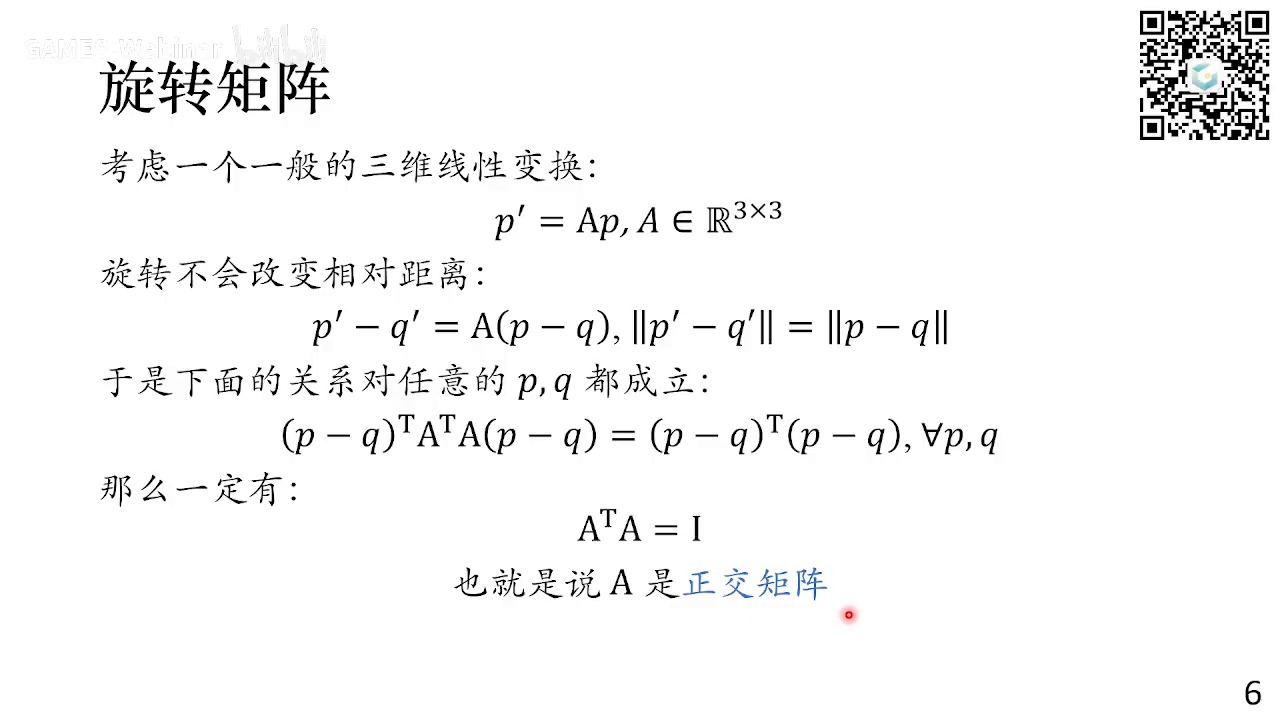
\includegraphics[width=0.92\textwidth]{figures/fig_03_rotation_matrix_derivation.jpg}
\caption{从“旋转不改变相对距离”推出 $\mathrm A^{\mathsf T}\mathrm A=\mathrm I$\vtag}
\end{figure}
\srcnote{00:04:30--00:04:45}
\end{minipage}


\subsection{正交矩阵不全是旋转}

讲者随机采样了一批正交矩阵作用在奶牛模型上，大多数结果看起来都是旋转。但正交矩阵的集合比旋转更大。例如
\[
\mathrm A=\begin{pmatrix}1&0&0\\0&1&0\\0&0&-1\end{pmatrix}
\]
也是正交矩阵，它把兔子模型关于 $xy$ 平面做了镜像。镜像后的兔子和原来的兔子有本质区别：无论怎么旋转，都不可能从原来的兔子得到镜像后的兔子。

\noindent\begin{minipage}{\textwidth}
\begin{figure}[H]
\centering
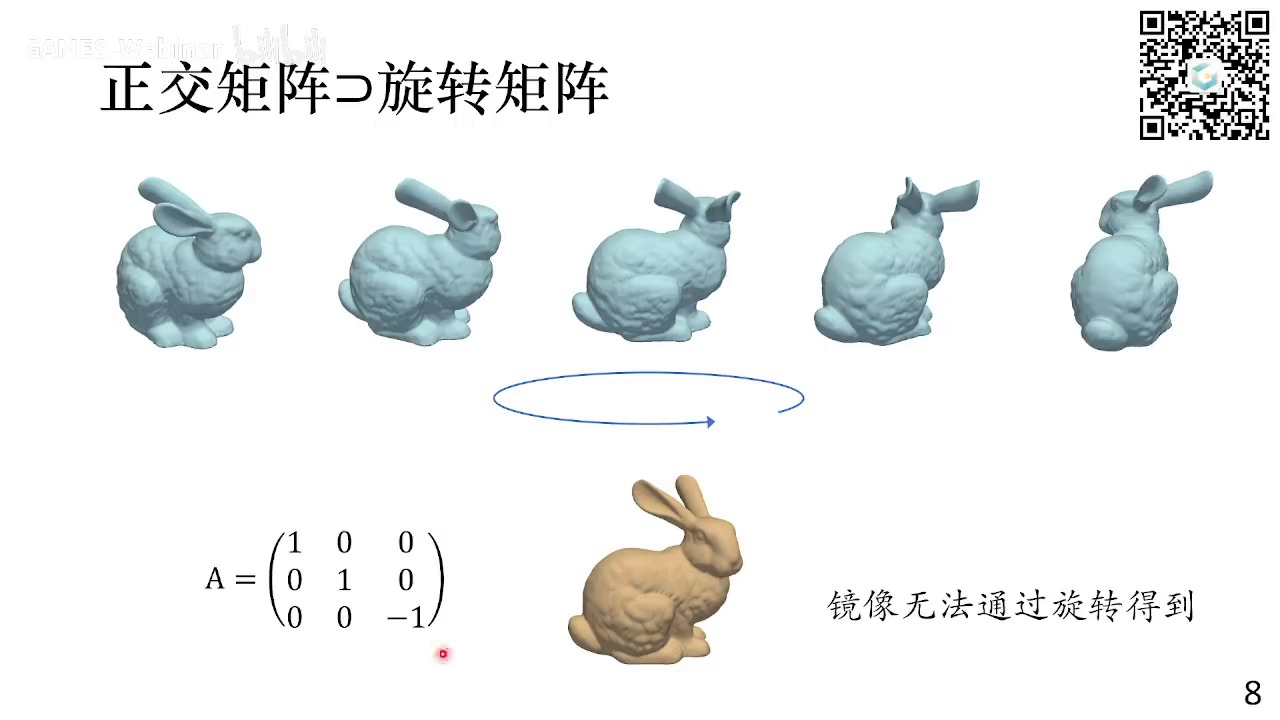
\includegraphics[width=0.92\textwidth]{figures/fig_04_mirror.jpg}
\caption{正交矩阵包含旋转矩阵：镜像也是正交变换，但无法通过旋转得到\vtag}
\end{figure}
\srcnote{00:05:45--00:06:00}
\end{minipage}


所以能够表示旋转的矩阵是正交矩阵中行列式为 $+1$ 的那一部分：
\[
\mathrm R^{\mathsf T}\mathrm R=\mathrm R\mathrm R^{\mathsf T}=\mathrm I,\qquad \det\mathrm R=1 .
\]
所有行列式为 $+1$ 的 $n$ 维正交矩阵构成的集合称为\textbf{特殊正交群}（special orthogonal group），记作 $SO(n)$。二维旋转矩阵的集合是 $SO(2)$，三维旋转矩阵的集合是 $SO(3)$。

\begin{warningbox}{“特征值为 $+1$”与“行列式为 $+1$”}
课件上写的是“特征值为 $+1$ 的正交矩阵”。讲义作者提醒：$SO(n)$ 的标准定义条件是 $\det\mathrm R=1$。三维中两者等价，因为行列式为 $+1$ 的 $3\times3$ 正交矩阵必有一个特征值为 $1$，对应的特征向量就是转轴；但在偶数维中，旋转矩阵可以没有实特征值，例如二维中转 $90^\circ$ 的矩阵。所以判断时应以行列式为准。
\end{warningbox}

\subsection{旋转群的性质}

既然旋转构成群，它就满足群的特征。

\begin{itemize}
\item \textbf{封闭性与结合律}：任意两个旋转相乘仍是旋转，并且
\[
\mathrm R=\mathrm R_2(\mathrm R_1\mathrm R_0)=(\mathrm R_2\mathrm R_1)\mathrm R_0 .
\]
课件中的例子是绕两个轴各转 $45^\circ$，合成后等价于绕 $\mathbf u=(0.67,0.67,0.28)$ 转 $\theta=62.8^\circ$ 的单次旋转。
\item \textbf{可逆性}：$\mathrm R^{-1}=\mathrm R^{\mathsf T}$，求逆只需转置。
\item \textbf{三维旋转不满足交换律}：$\mathrm R_1\mathrm R_0\neq\mathrm R_0\mathrm R_1$。
\end{itemize}

\noindent\begin{minipage}{\textwidth}
\begin{figure}[H]
\centering
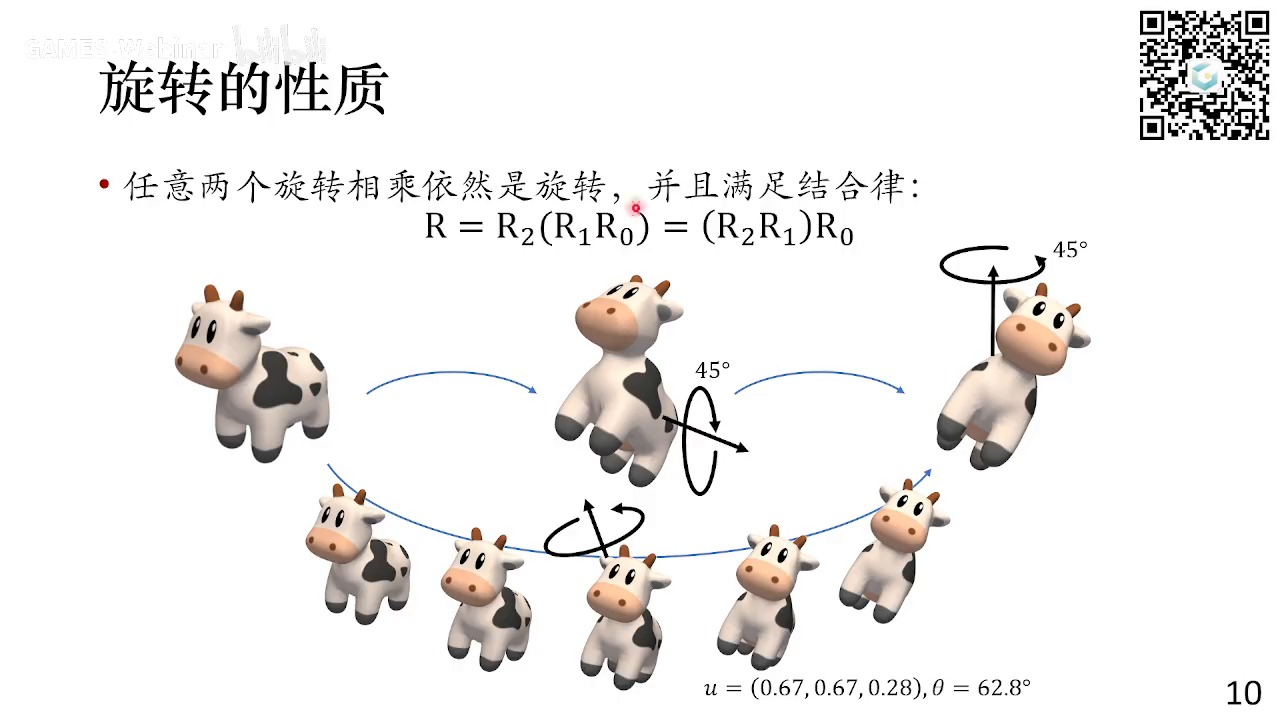
\includegraphics[width=0.92\textwidth]{figures/fig_05_composition.jpg}
\caption{旋转的复合：两次 $45^\circ$ 旋转合成为绕 $\mathbf u=(0.67,0.67,0.28)$ 的 $62.8^\circ$ 旋转\vtag}
\end{figure}
\srcnote{00:08:00--00:08:15}
\end{minipage}


二维旋转是可交换的：先转 $10^\circ$ 再转 $20^\circ$，与先转 $20^\circ$ 再转 $10^\circ$ 结果相同。三维则不然。原因在于三维旋转还有“旋转轴”的概念：两次旋转的轴不同时，先转哪一个会改变第二次旋转所面对的物体朝向。课件上的例子是：先绕 $x$ 轴转 $90^\circ$、再绕 $y$ 轴转 $90^\circ$，与先绕 $y$ 轴转 $90^\circ$、再绕 $x$ 轴转 $90^\circ$，奶牛最后的朝向不同。

\noindent\begin{minipage}{\textwidth}
\begin{figure}[H]
\centering
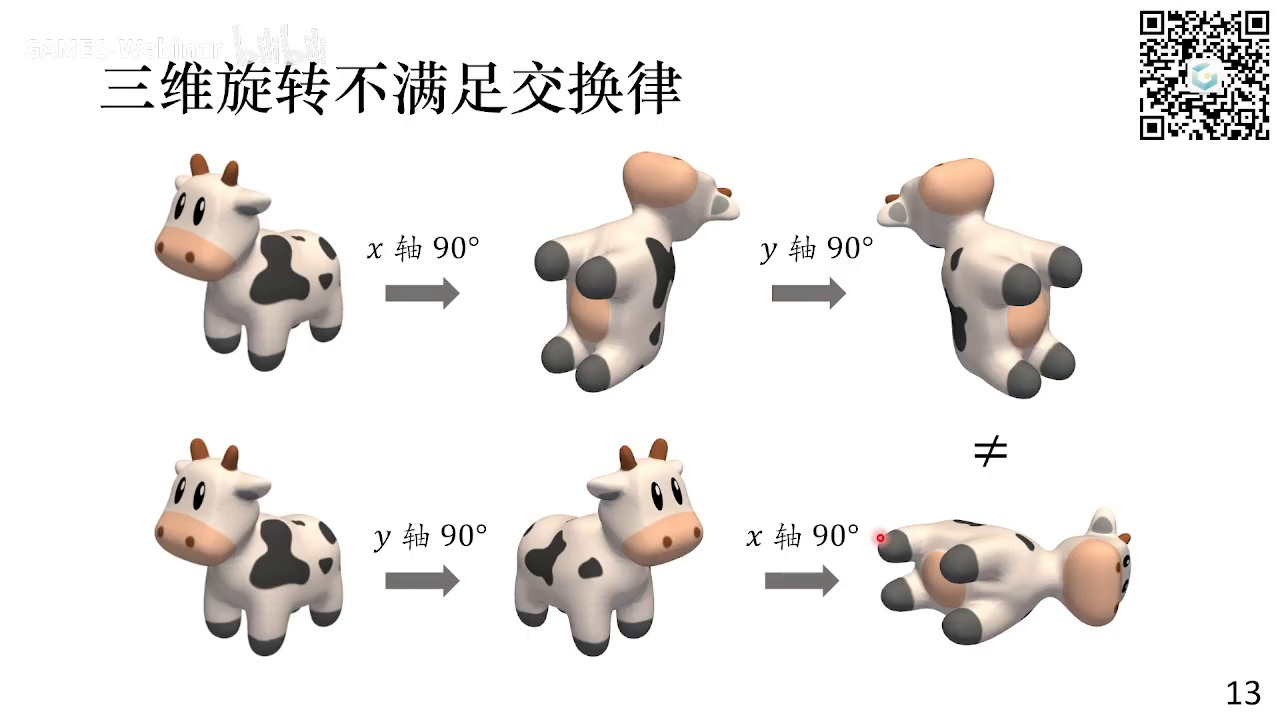
\includegraphics[width=0.92\textwidth]{figures/fig_06_noncommutative.jpg}
\caption{三维旋转不满足交换律：$x$ 轴 $90^\circ$ 再 $y$ 轴 $90^\circ$ 不等于反过来的顺序\vtag}
\end{figure}
\srcnote{00:09:45--00:10:00}
\end{minipage}


\section{为什么要研究旋转的表示}

\subsection{图形学中的四个现实问题}

旋转矩阵有 9 个数，但直接用它来解决问题往往不方便。讲者列出四个现实问题：

\begin{enumerate}
\item \textbf{相机交互}：鼠标在屏幕上的移动轨迹是二维的，只有 $x$ 和 $y$ 方向的位移，而旋转矩阵有 9 个数。如何把屏幕空间里鼠标的位移 $(\Delta x,\Delta y)$ 映射成相机视角的旋转 $\mathrm R\leftarrow F(\Delta x,\Delta y)$？
\item \textbf{关键帧插值}：角色动画里，动画师只给出若干关键帧上的关节旋转，如何从关键帧 $\mathrm R_0,\mathrm R_1$ 插值出中间的旋转 $\mathrm R(t)\leftarrow F(\mathrm R_0,\mathrm R_1,t)$？
\item \textbf{物理模拟}：刚体动力学方程用角速度（角动量）建立，但最终要得到刚体的旋转。角速度 $\boldsymbol\omega$ 与旋转 $\mathrm R$ 是什么关系？
\item \textbf{机器学习}：神经网络如何学习、估计或生成旋转？
\end{enumerate}

\noindent\begin{minipage}{\textwidth}
\begin{figure}[H]
\centering
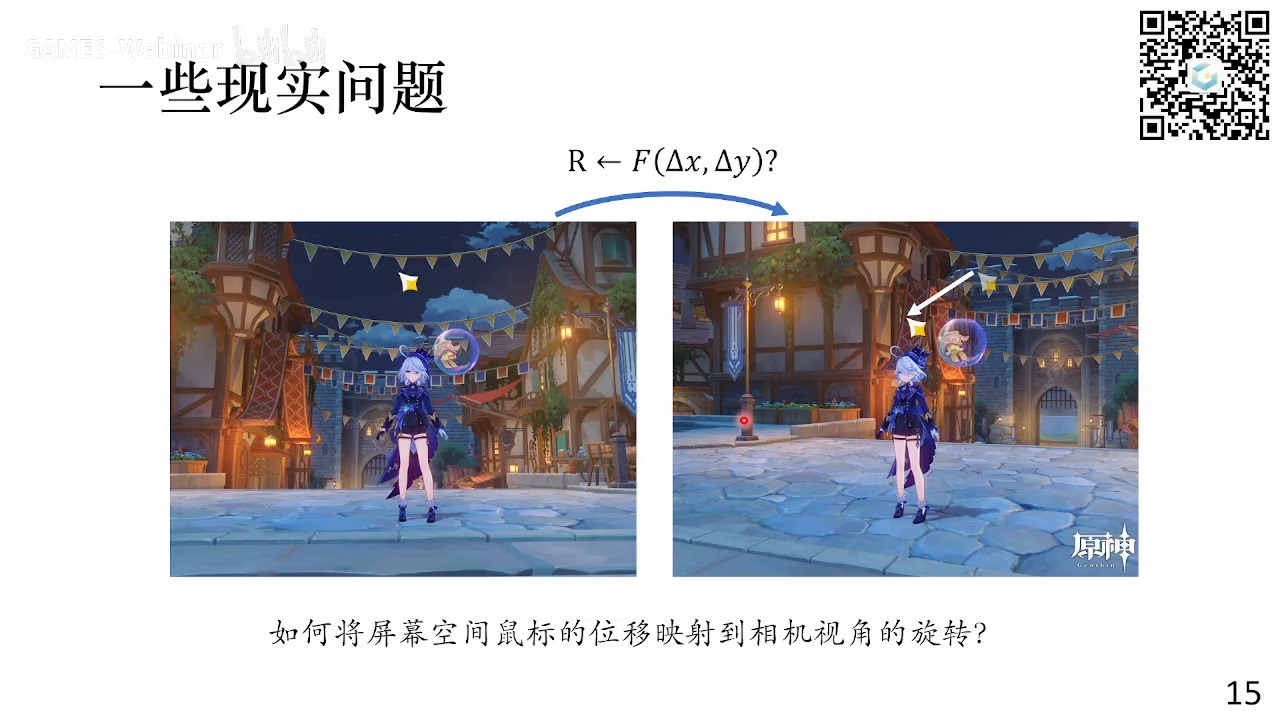
\includegraphics[width=0.92\textwidth]{figures/fig_07_problem_mouse.jpg}
\caption{现实问题之一：如何把鼠标位移映射为相机旋转\vtag}
\end{figure}
\srcnote{00:10:45--00:11:00}
\end{minipage}


\noindent\begin{minipage}{\textwidth}
\begin{figure}[H]
\centering
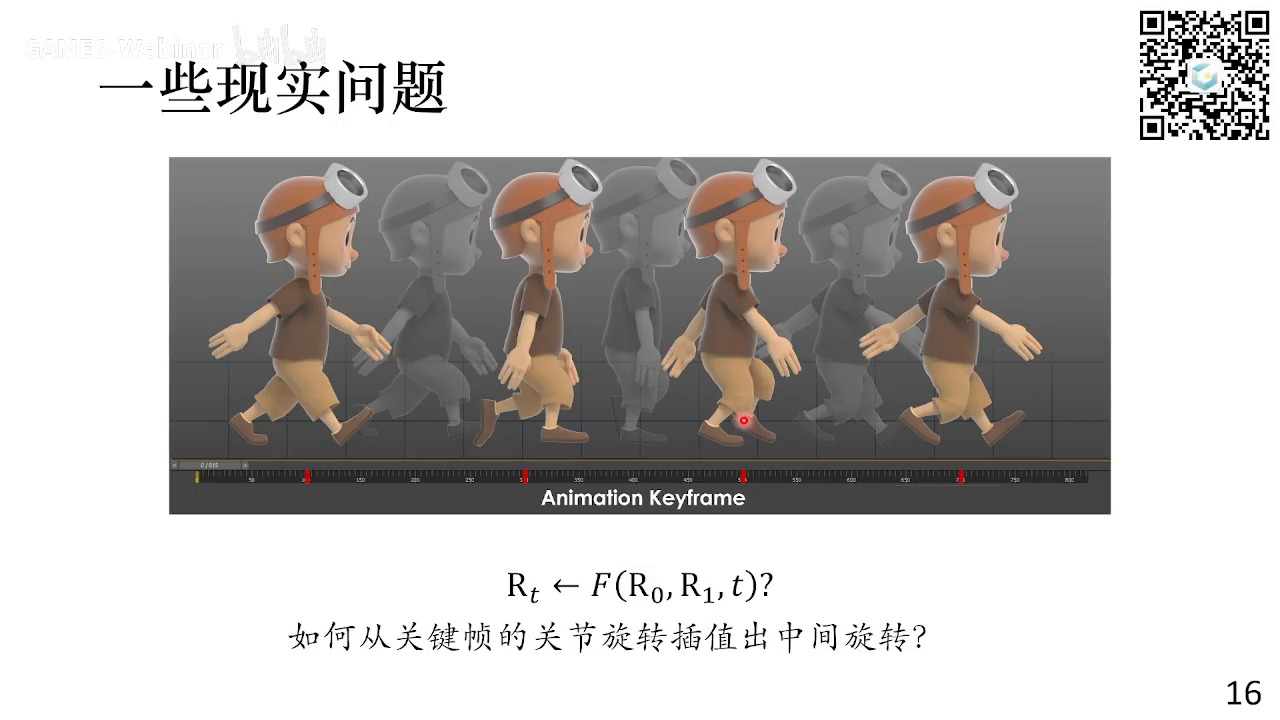
\includegraphics[width=0.92\textwidth]{figures/fig_08_problem_keyframe.jpg}
\caption{现实问题之二：如何在关键帧之间插值关节旋转\vtag}
\end{figure}
\srcnote{00:11:30--00:11:45}
\end{minipage}


\noindent\begin{minipage}{\textwidth}
\begin{figure}[H]
\centering
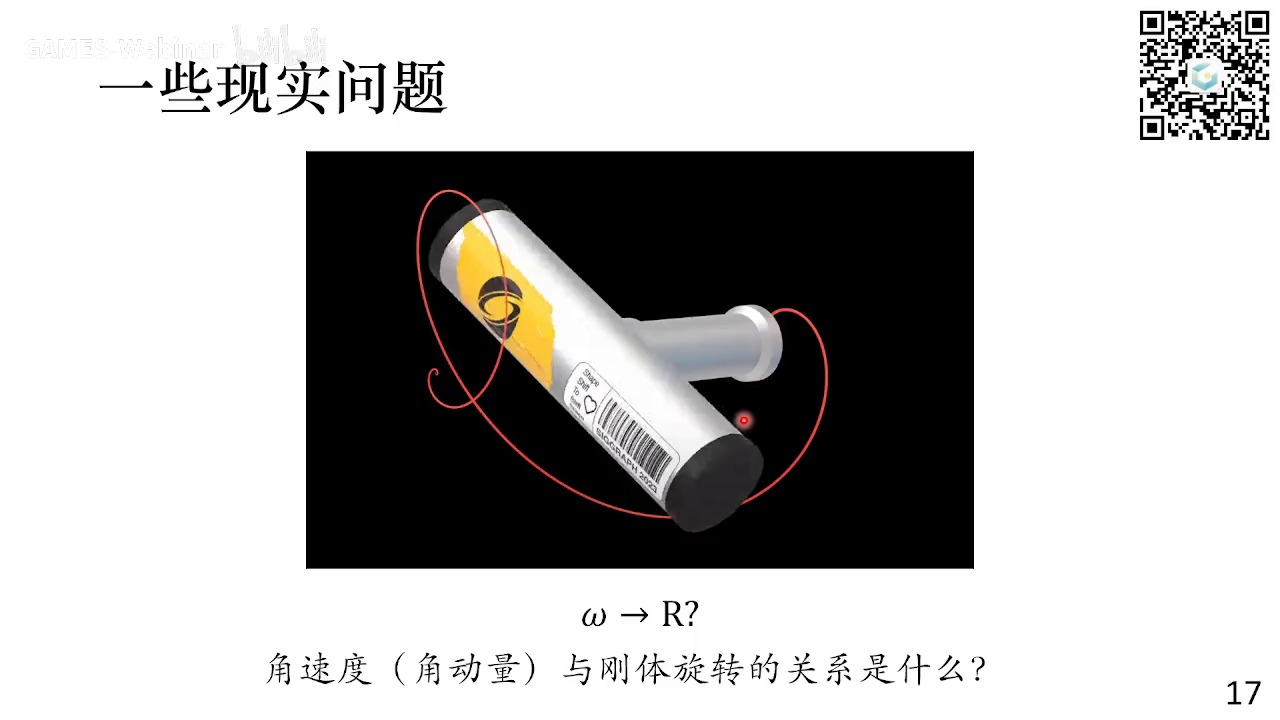
\includegraphics[width=0.92\textwidth]{figures/fig_09_problem_angvel.jpg}
\caption{现实问题之三：角速度与刚体旋转的关系\vtag}
\end{figure}
\srcnote{00:12:15--00:12:30}
\end{minipage}


这些问题的共同点是：要在计算机里\emph{参数化}旋转，再用参数化后的旋转完成任务。

\subsection{旋转的自由度}

要参数化旋转，先要知道它有几个自由度。二维旋转只需一个角度 $\theta\in\mathbb R$，自由度为 1。三维旋转可以用一个单位转轴 $\mathbf u\in\mathbb R^3$、$\|\mathbf u\|=1$ 和一个角度 $\theta\in\mathbb R$ 描述；$\mathbf u$ 只有方向有用，长度被约束掉了，所以自由度是 $2+1=3$。

\noindent\begin{minipage}{\textwidth}
\begin{figure}[H]
\centering
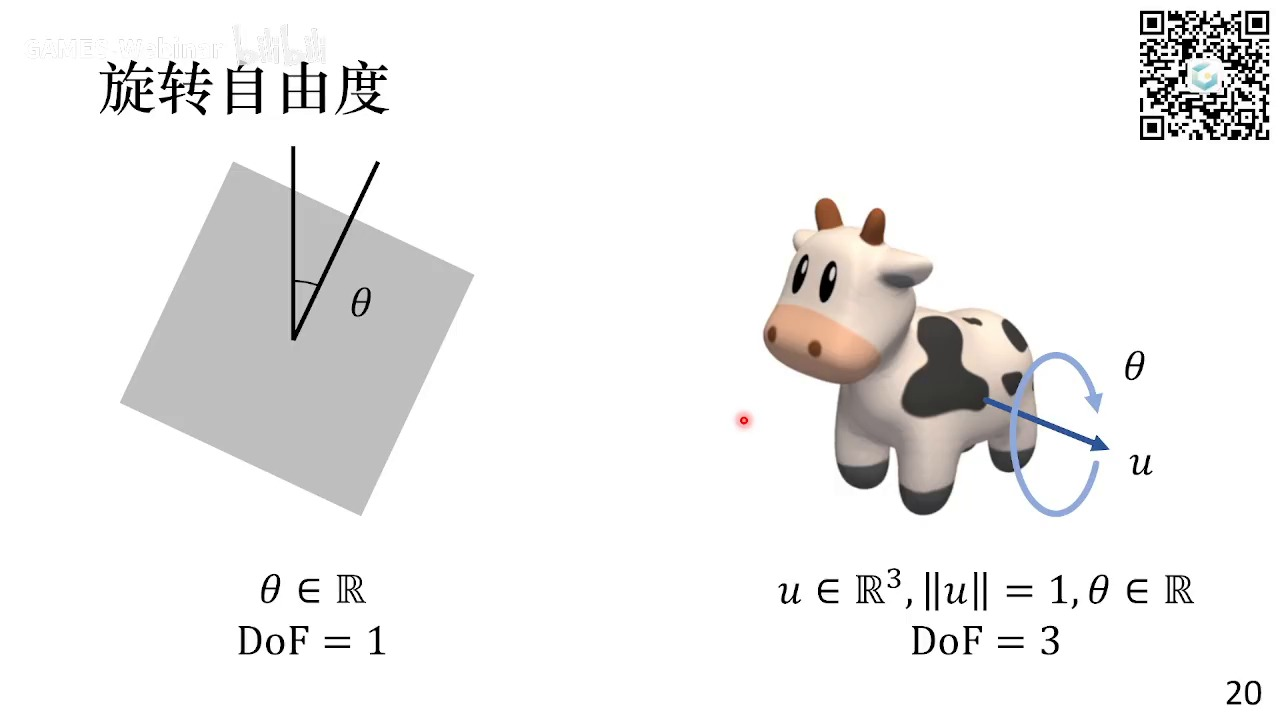
\includegraphics[width=0.92\textwidth]{figures/fig_10_dof.jpg}
\caption{旋转的自由度：二维为 1，三维为转轴方向 2 个加角度 1 个\vtag}
\end{figure}
\srcnote{00:15:15--00:15:30}
\end{minipage}


从矩阵的角度数约束也得到同样的结论。二维时，$\mathrm R^{\mathsf T}\mathrm R=\mathrm I$ 给出两个对角元条件和一个非对角元条件：
\[
\mathrm R_{00}^2+\mathrm R_{01}^2=1,\qquad
\mathrm R_{10}^2+\mathrm R_{11}^2=1,\qquad
\mathrm R_{00}\mathrm R_{10}+\mathrm R_{01}\mathrm R_{11}=0,
\]
自由度为 $4-3=1$。三维时有 3 个模长条件和 3 个正交条件，共 6 个约束，自由度为 $9-6=3$。

\noindent\begin{minipage}{\textwidth}
\begin{figure}[H]
\centering
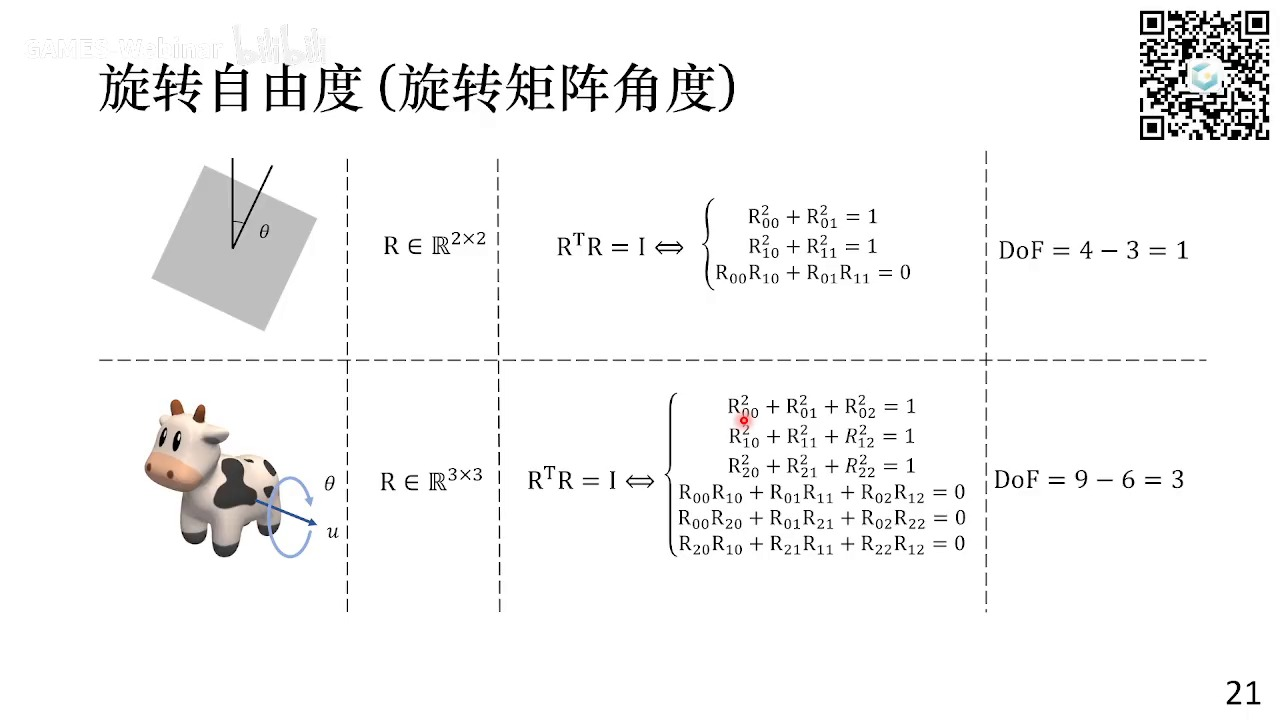
\includegraphics[width=0.92\textwidth]{figures/fig_11_dof_matrix.jpg}
\caption{用矩阵约束计数：二维 $4-3=1$，三维 $9-6=3$\vtag}
\end{figure}
\srcnote{00:17:00--00:17:15}
\end{minipage}


\subsection{流形与李群}

讲者用流形（manifold）来理解“旋转所在的空间”。圆是二维空间中的一维流形：它在局部看起来像一条线段，但整体上无法展开成一条直线。球面是三维空间中的二维流形；克莱因瓶等也都是流形的例子。

二维旋转矩阵 $\mathrm R\in\mathbb R^{2\times2}$ 有 4 个数、1 个自由度，所以所有二维旋转构成 4 维空间中的 1 维流形；三维旋转矩阵 $\mathrm R\in\mathbb R^{3\times3}$ 有 9 个数、3 个自由度，构成 9 维空间中的 3 维流形。

讲者解释“几维空间中的几维流形”时，用了两个层次。第一个数字是“画出它需要的空间”：克莱因瓶是画在三维空间里的模型，所以说它在三维空间中。第二个数字是“局部看起来像什么”：离克莱因瓶的任意一点足够近，局部看它都是一小片平面，所以它是二维流形。圆也是如此：局部看是一小段线段，所以是一维流形；但它首尾相接，没有办法整个展开成一条直线，只有在二维空间里才画得出来。旋转流形同理：所有二维旋转矩阵作为 4 维空间中的点，连起来局部像一条线；所有三维旋转矩阵作为 9 维空间中的点，局部像一块三维的区域。

\noindent\begin{minipage}{\textwidth}
\begin{figure}[H]
\centering
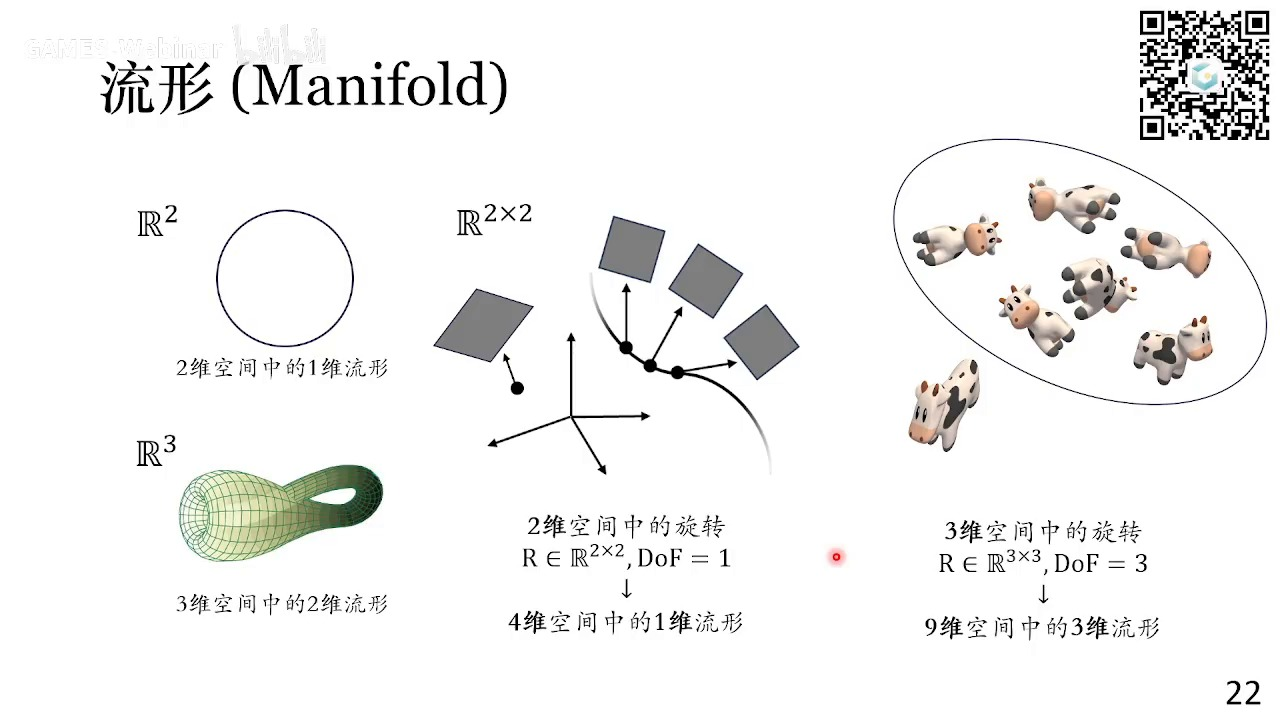
\includegraphics[width=0.92\textwidth]{figures/fig_12_manifold.jpg}
\caption{流形：圆、球面，以及“二维旋转是 4 维空间中的 1 维流形，三维旋转是 9 维空间中的 3 维流形”\vtag}
\end{figure}
\srcnote{00:21:15--00:21:30}
\end{minipage}


一个对象如果既是群又是流形，就称为\textbf{李群}（Lie group）：群 $+$ 流形 $=$ 李群。机器人学和状态估计等领域的文献里，经常用李群的语言来处理旋转。

\noindent\begin{minipage}{\textwidth}
\begin{figure}[H]
\centering
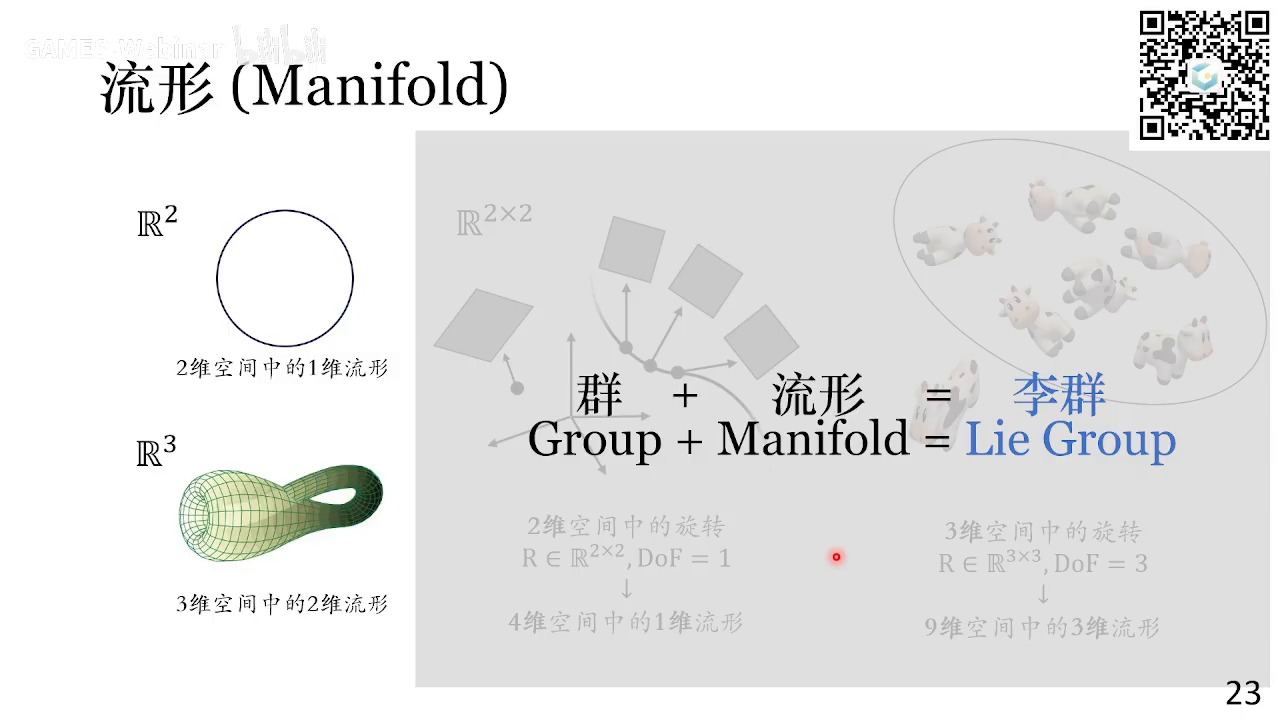
\includegraphics[width=0.92\textwidth]{figures/fig_13_liegroup.jpg}
\caption{群 $+$ 流形 $=$ 李群\vtag}
\end{figure}
\srcnote{00:22:30--00:22:45}
\end{minipage}


\subsection{插值与角速度的流形视角}

流形视角立即解释了一个常见错误：直接对旋转矩阵做线性插值
\[
\mathrm R(t)=(1-t)\mathrm R_0+t\mathrm R_1
\]
得到的 $\mathrm R(t)$ 一般不在旋转流形上，不再是正交矩阵，奶牛会被拉伸变形。正确的做法是沿着流形上的路径从 $\mathrm R_0$ 走到 $\mathrm R_1$，并且路径越短越好，因为最短的路径意味着中间的变化最小，插值最自然。

\noindent\begin{minipage}{\textwidth}
\begin{figure}[H]
\centering
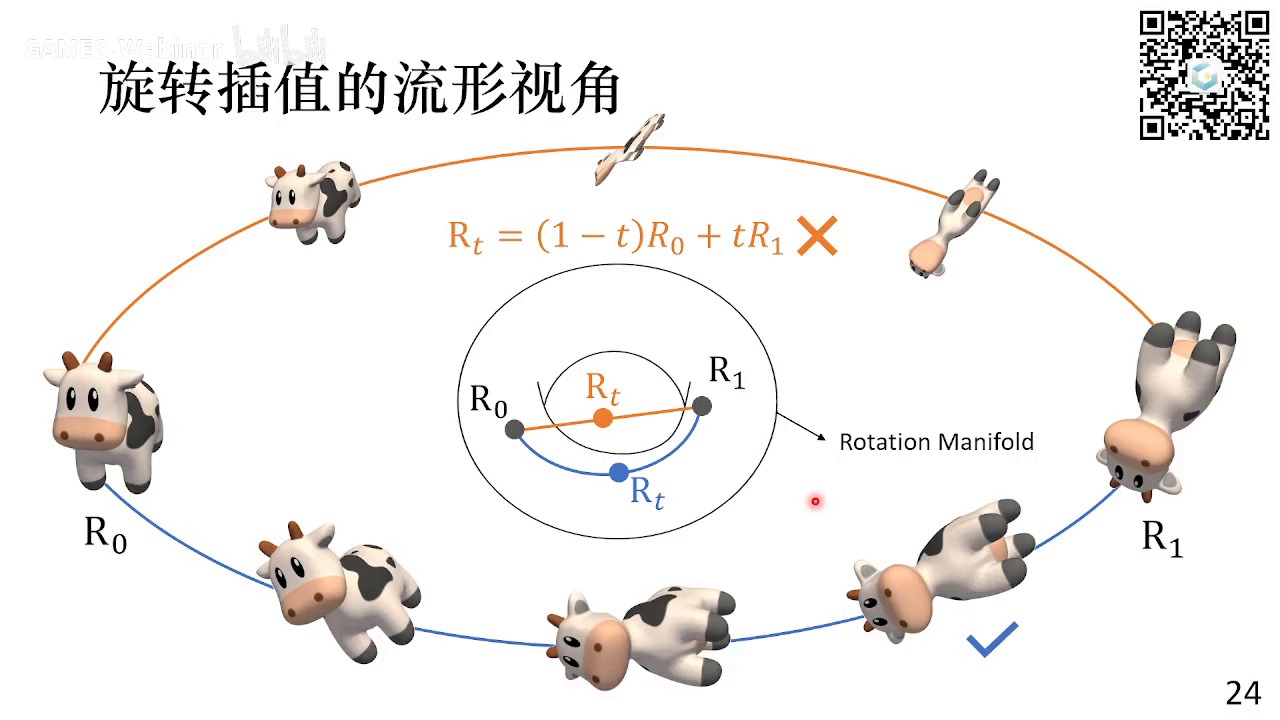
\includegraphics[width=0.92\textwidth]{figures/fig_14_interp_manifold.jpg}
\caption{旋转插值的流形视角：线性插值离开流形（$\times$），应沿流形上的测地线插值（$\checkmark$）\vtag}
\end{figure}
\srcnote{00:24:15--00:24:30}
\end{minipage}


流形视角也有助于理解角速度。欧氏空间中，点沿轨迹运动，速度 $\mathbf v=\mathrm d\mathbf x/\mathrm dt\in\mathbb R^3$。对旋转矩阵直接求导，得到的 $\mathrm d\mathrm R/\mathrm dt$ 是 $3\times3$ 矩阵；而角速度 $\boldsymbol\omega$ 是三维矢量，二者显然不是直接相等的关系。什么东西是三维的？旋转流形在任意一点的切空间 $\mathcal T_{x}\mathcal M\cong\mathbb R^3$。角速度正是活在切空间里的量，本讲最后一节会给出它与 $\dot{\mathrm R}$ 的精确关系。

\noindent\begin{minipage}{\textwidth}
\begin{figure}[H]
\centering
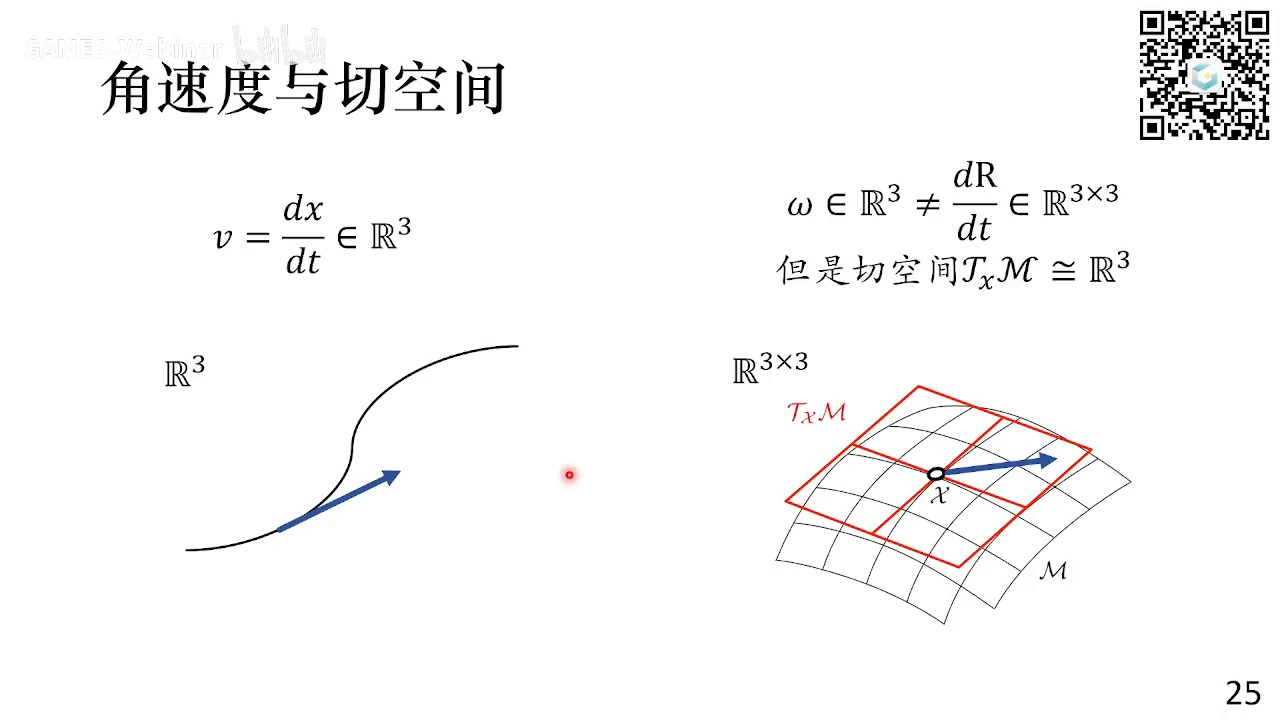
\includegraphics[width=0.92\textwidth]{figures/fig_15_tangent.jpg}
\caption{角速度与切空间：$\mathrm d\mathrm R/\mathrm dt\in\mathbb R^{3\times3}$，但切空间 $\mathcal T_x\mathcal M\cong\mathbb R^3$\vtag}
\end{figure}
\srcnote{00:25:45--00:26:00}
\end{minipage}


\begin{knowledgebox}{旋转表示 $=$ 流形参数化}
旋转流形是嵌在 9 维空间里的 3 维曲面。所谓“旋转表示”，就是给这个流形找一套坐标：用若干个参数（欧拉角 3 个、轴角 3 个、四元数 4 个、6D 表示 6 个等）去对应流形上的点。不同参数化在直观性、奇异性、插值和计算效率上各有取舍，下面逐一比较。

讲者用 GAMES101 中的纹理映射作类比：一个奇形怪状的三维模型要贴上贴图，就要给模型表面每个点分配一个二维的 $(u,v)$ 坐标，也就是把三维模型上的二维曲面“摊”到二维平面上。旋转表示做的是同一件事：把 9 维空间中的 3 维旋转流形映射到一个 3 维（或稍高维）的参数空间。参数化之后，对旋转求导、优化时面对的是少数几个参数，而不是带约束的 $3\times3$ 矩阵。
\end{knowledgebox}

\noindent\begin{minipage}{\textwidth}
\begin{figure}[H]
\centering
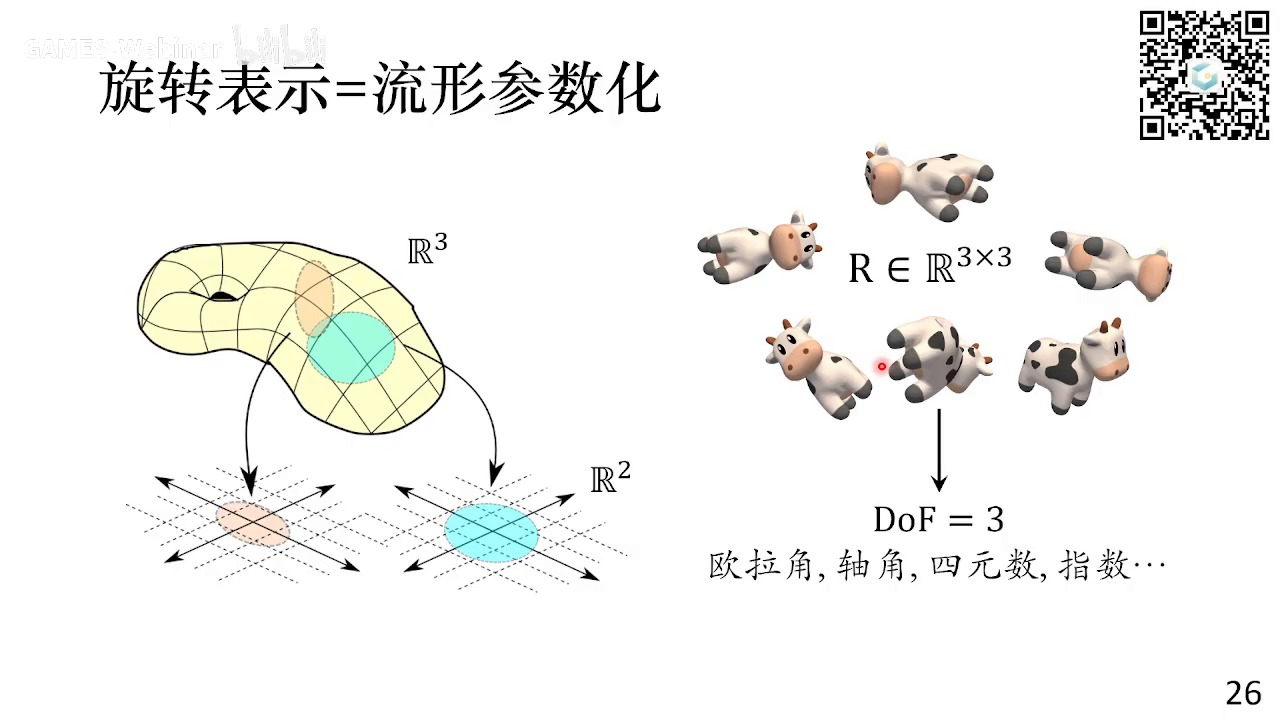
\includegraphics[width=0.92\textwidth]{figures/fig_16_param.jpg}
\caption{旋转表示即流形参数化：用低维参数覆盖 $\mathbb R^{3\times3}$ 中的 3 维旋转流形\vtag}
\end{figure}
\srcnote{00:27:15--00:27:30}
\end{minipage}


\section{欧拉角}

\subsection{旋转与坐标变换}

在介绍欧拉角之前，讲者先澄清旋转与坐标变换的关系。对于旋转前的一个点 $\mathbf p$，旋转后有两种表示方法：在世界坐标系下的坐标 $\mathbf p'_w$，以及在跟随物体旋转的局部坐标系下的坐标 $\mathbf p'_l$。由于局部坐标系随物体一起转，点在局部坐标系下没动，$\mathbf p'_l=\mathbf p$。只在世界坐标系下考虑，有 $\mathbf p'_w=\mathrm R\mathbf p$；也可以理解为
\[
\mathbf p'_w=\mathrm R\,\mathbf p'_l ,
\]
即 $\mathrm R$ 表示的是\emph{从局部坐标系到世界坐标系}的坐标变换。做渲染时经常需要在不同坐标系之间换算，这个理解非常有用。

\noindent\begin{minipage}{\textwidth}
\begin{figure}[H]
\centering
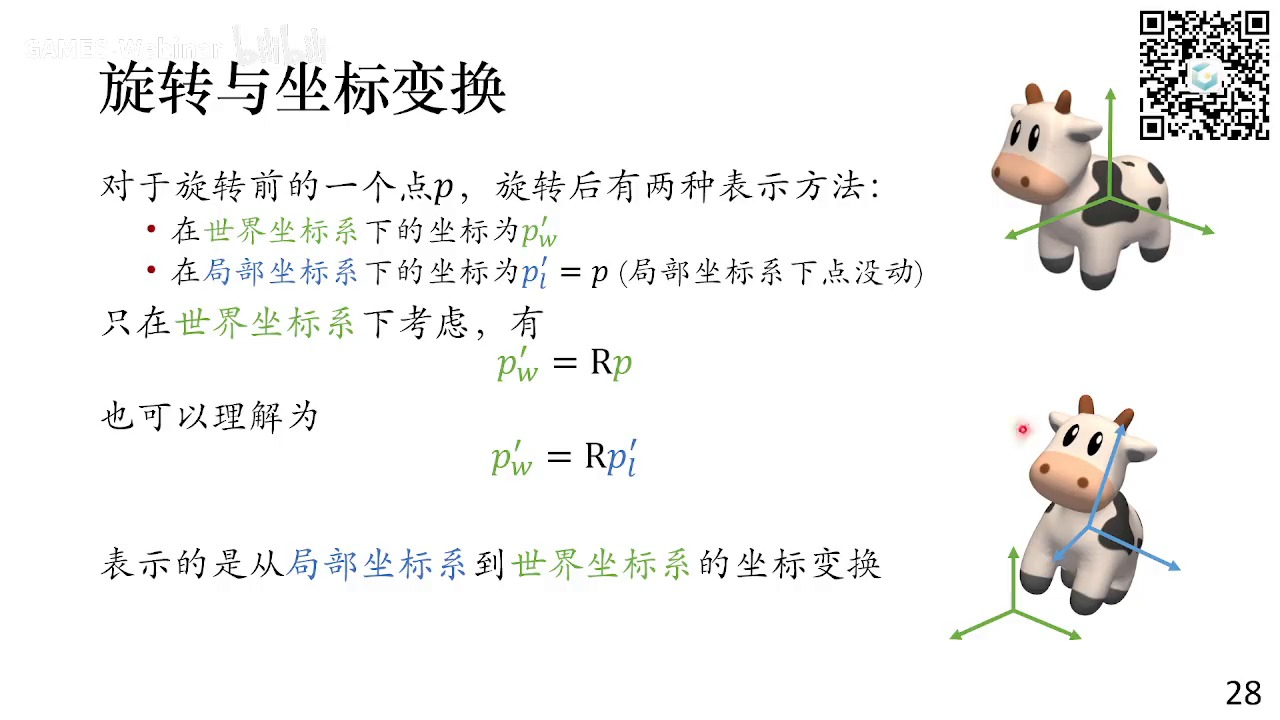
\includegraphics[width=0.92\textwidth]{figures/fig_17_coord_transform.jpg}
\caption{旋转与坐标变换：$\mathrm R$ 把局部坐标变换到世界坐标\vtag}
\end{figure}
\srcnote{00:31:15--00:31:30}
\end{minipage}


\subsection{三次旋转的复合}

欧拉角把任意旋转分解为绕坐标轴的三次旋转，参数为 $(\alpha,\beta,\gamma)\in\mathbb R^3$。以课件中的 $Z$--$X$--$Z$ 顺序为例，每次旋转后都得到一个新的局部坐标系，点在第三个局部坐标系下的坐标为 $\mathbf x_{l3}$，则
\[
\mathbf x_w=\mathrm R_1\mathbf x_{l1}=\mathrm R_1\mathrm R_2\mathbf x_{l2}=\mathrm R_1\mathrm R_2\mathrm R_3\mathbf x_{l3},\qquad
\mathrm R=Z(\alpha)X(\beta)Z(\gamma),
\]
其中
\[
Z(\alpha)=\begin{pmatrix}\cos\alpha&-\sin\alpha&0\\ \sin\alpha&\cos\alpha&0\\0&0&1\end{pmatrix},\qquad
X(\beta)=\begin{pmatrix}1&0&0\\0&\cos\beta&-\sin\beta\\0&\sin\beta&\cos\beta\end{pmatrix}.
\]
有同学在弹幕里问：为什么后一次旋转是乘在右边，而不是乘在 $\mathrm R_1$ 的左边？答案就在上面的坐标变换链：每一次旋转都是绕\emph{当前局部坐标系}的轴进行的，所以要把新的局部到旧局部的变换接在右边。

\noindent\begin{minipage}{\textwidth}
\begin{figure}[H]
\centering
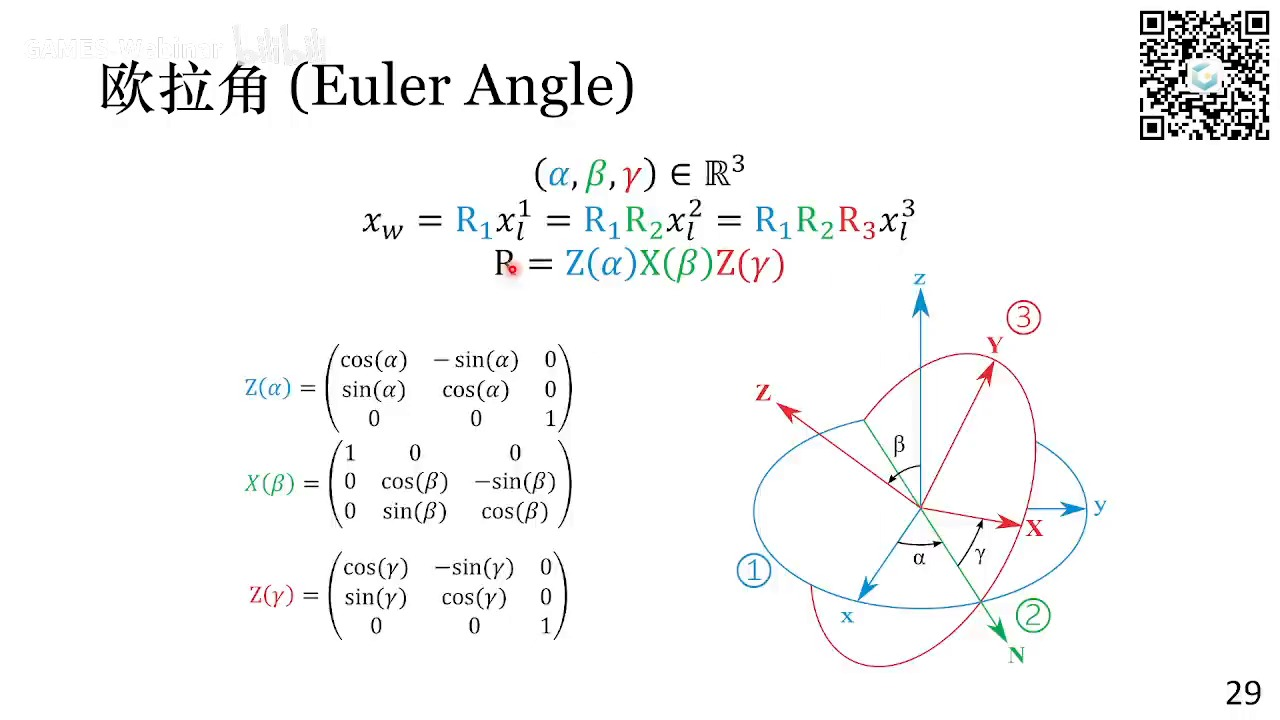
\includegraphics[width=0.92\textwidth]{figures/fig_18_euler.jpg}
\caption{欧拉角 $Z(\alpha)X(\beta)Z(\gamma)$：三次绕局部坐标轴的旋转及对应的矩阵\vtag}
\end{figure}
\srcnote{00:35:45--00:36:00}
\end{minipage}


三次旋转的顺序可以自由选择，如 $XZX$、$XYX$、$XYZ$、$ZYX$ 等，维基百科等资料里列出了每种组合对应的旋转矩阵，方便查表。但不同顺序得到的结果互不相同，因为旋转群不满足交换律。使用欧拉角时，必须先约定顺序。

\noindent\begin{minipage}{\textwidth}
\begin{figure}[H]
\centering
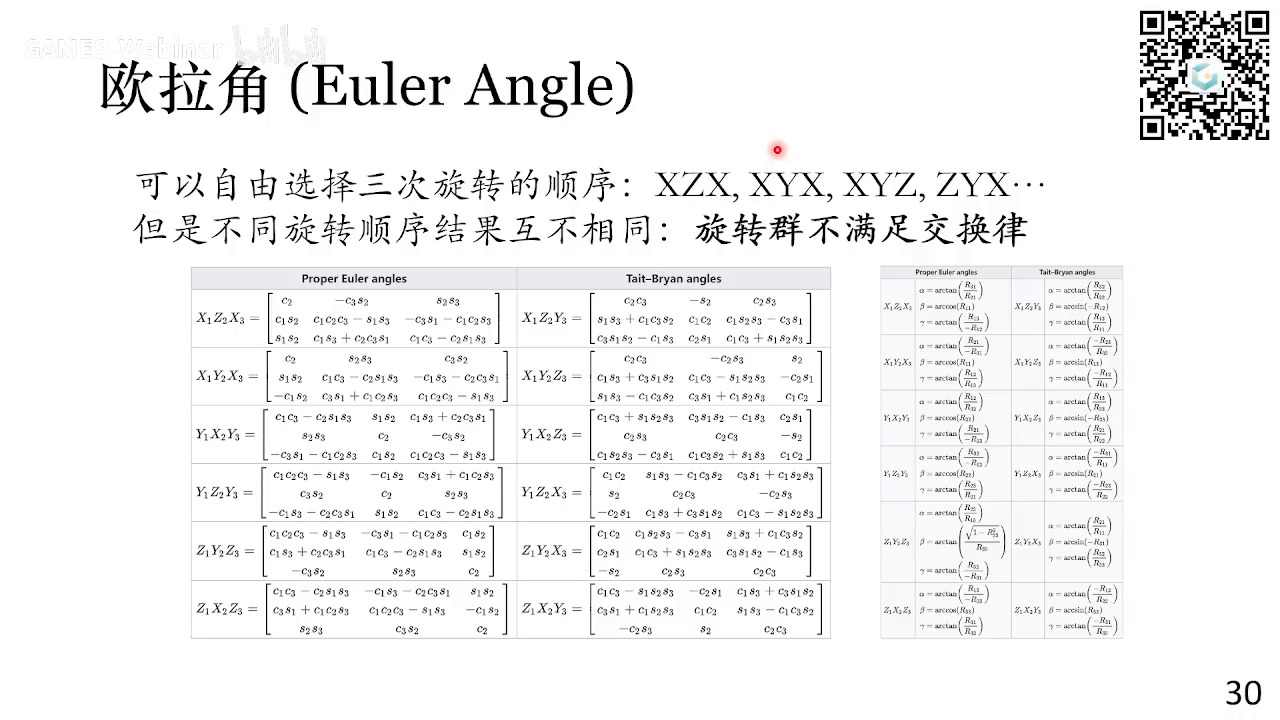
\includegraphics[width=0.92\textwidth]{figures/fig_19_euler_orders.jpg}
\caption{欧拉角的旋转顺序可以自由选择，但不同顺序的结果互不相同\vtag}
\end{figure}
\srcnote{00:37:00--00:37:15}
\end{minipage}


\subsection{内旋与外旋}

如果每次旋转都绕\emph{随物体转动后的}局部坐标轴进行，称为\textbf{内旋}（intrinsic rotations）；如果每次都绕最外面固定的世界坐标轴进行，称为\textbf{外旋}（extrinsic rotations）。讲者把“内旋与外旋的关系是什么”留作作业，提示推导用到的正是刚才的坐标变换。

\begin{knowledgebox}{作业提示：内旋与外旋}
讲义作者补充一个结论供核对：按 $Z$--$X$--$Z$ 顺序绕局部轴的内旋 $(\alpha,\beta,\gamma)$，等价于按相反顺序 $Z$--$X$--$Z$ 绕世界轴的外旋 $(\gamma,\beta,\alpha)$，二者的矩阵都是 $Z(\alpha)X(\beta)Z(\gamma)$。内旋把后面的旋转右乘，外旋把后面的旋转左乘，所以“顺序反过来”恰好抵消。
\end{knowledgebox}

\noindent\begin{minipage}{\textwidth}
\begin{figure}[H]
\centering
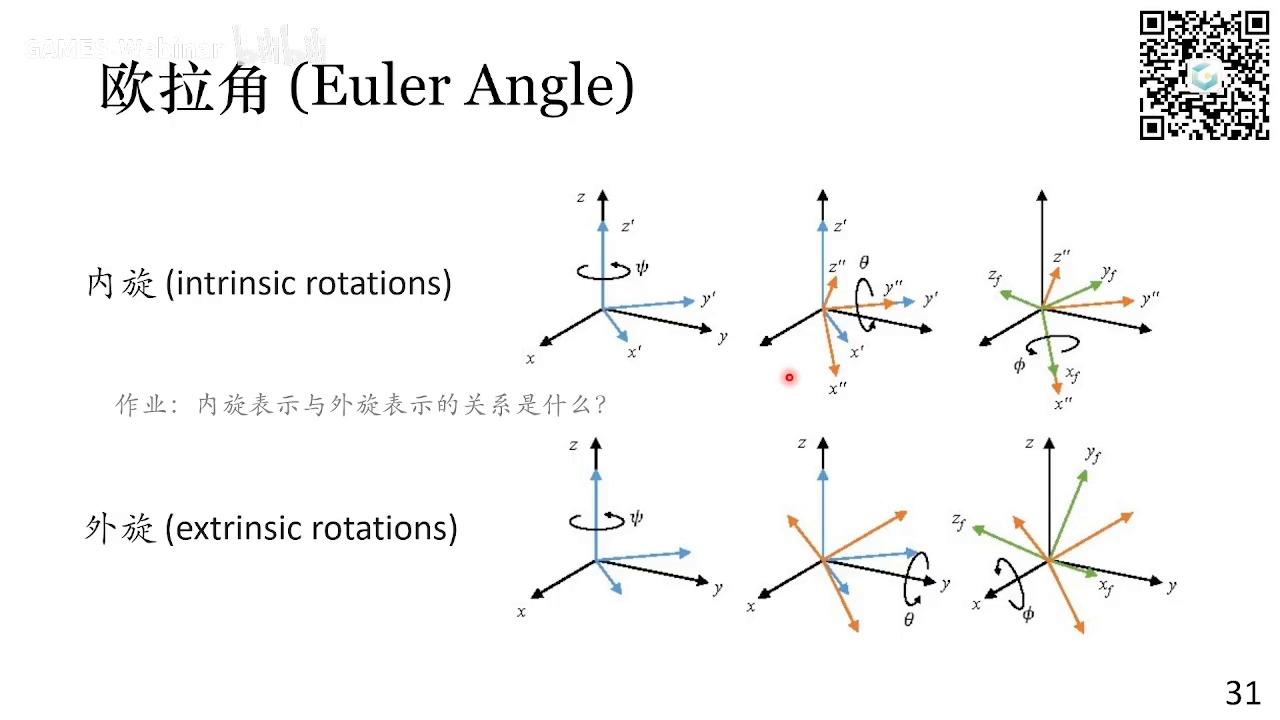
\includegraphics[width=0.92\textwidth]{figures/fig_20_intrinsic_extrinsic.jpg}
\caption{内旋（绕局部轴）与外旋（绕世界轴）\vtag}
\end{figure}
\srcnote{00:39:30--00:39:45}
\end{minipage}


\subsection{航向、俯仰、横滚}

欧拉角在工程上最常见的规范来自航空业，三个角各有具体含义：\textbf{航向}（yaw）、\textbf{俯仰}（pitch）和\textbf{横滚}（roll）。游戏里的第一人称相机通常只用航向和俯仰：鼠标左右移动改变航向，上下移动改变俯仰，一般不需要横滚，否则相机翻转会让人头晕。这正好回答了前面“鼠标位移如何映射为相机旋转”的问题。欧拉角的最大优点就是直观：三个角各管一件事，动画师和用户都容易理解和调节。Blender 的物体属性面板中，旋转默认也是用欧拉角显示和编辑的。

\noindent\begin{minipage}{\textwidth}
\begin{figure}[H]
\centering
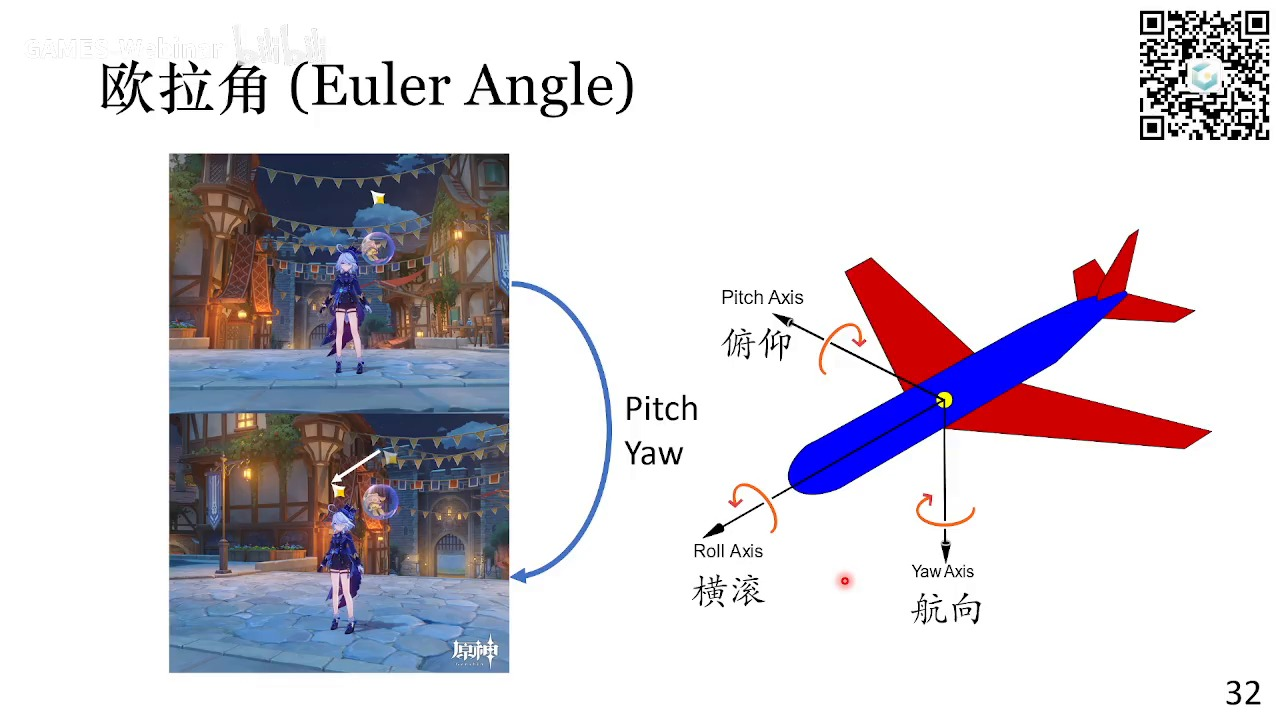
\includegraphics[width=0.92\textwidth]{figures/fig_21_pitch_yaw.jpg}
\caption{航向、俯仰、横滚：欧拉角的航空规范与游戏相机\vtag}
\end{figure}
\srcnote{00:41:00--00:41:15}
\end{minipage}


\subsection{万向锁}

欧拉角非常直观，但它有一个致命问题：\textbf{万向锁}（gimbal lock）。当航向轴与俯仰轴平行时，改变横滚角的效果与改变航向角完全相同。在这个特殊的点上，欧拉角只能调节 2 个自由度的旋转，有 1 个自由度被锁住了。俯仰角等于 $\pi/2$ 就是这样一个奇点（singularity）。

讲者用课件右下角的万向节（gimbal）动画说明：三个嵌套的圆环分别对应航向、俯仰、横滚。当紫色的航向环和绿色的俯仰环转到平行时，无论转动蓝色的环还是外面紫色的环，飞机做的都是同一个横滚动作。明明有三个参数，在这个点上却只能控制两个方向，剩下一个方向被“锁”住了。如果希望在这个点附近旋转是连续可控的，就需要额外的处理，这在动画和控制中都是很严重的问题。

\noindent\begin{minipage}{\textwidth}
\begin{figure}[H]
\centering
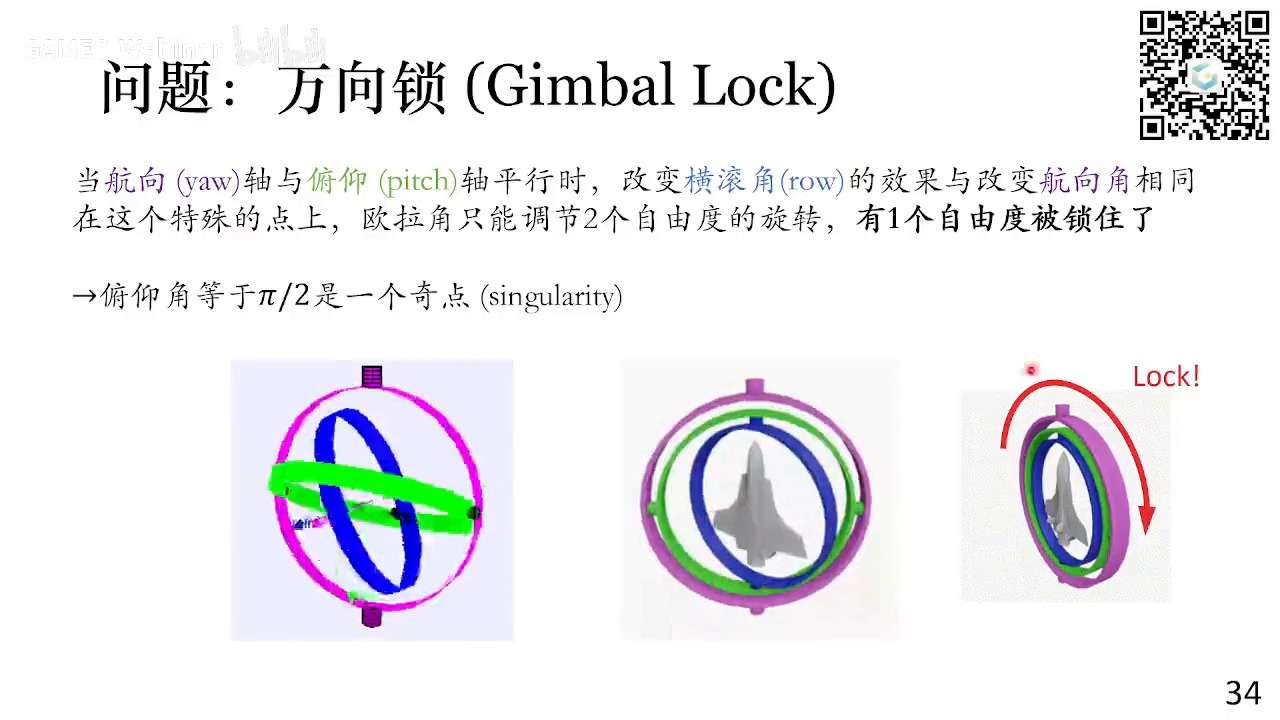
\includegraphics[width=0.92\textwidth]{figures/fig_22_gimbal.jpg}
\caption{万向锁：俯仰角为 $\pi/2$ 时，两个转轴重合，损失一个自由度\vtag}
\end{figure}
\srcnote{00:43:00--00:43:15}
\end{minipage}


\begin{warningbox}{三个参数不等于三个自由度}
欧拉角用三个参数表达三维流形，但在奇点附近，参数到旋转的映射退化了：两个参数的变化产生同样的旋转。这不是实现问题，而是用 $\mathbb R^3$ 的一张“坐标图”覆盖 $SO(3)$ 时必然出现的拓扑障碍。所以在插值、优化或物理模拟中，欧拉角常常会在奇点附近出现跳变或数值不稳定。
\end{warningbox}

\section{轴角与罗德里格旋转公式}

\subsection{轴角表示}

轴角表示（axis angle）直接用旋转的定义：旋转轴 $\mathbf u\in\mathbb R^3$，$\|\mathbf u\|=1$，以及旋转角度 $\theta\in\mathbb R$。两者也可以合成一个\textbf{旋转向量}
\[
\boldsymbol\theta=\theta\mathbf u\in\mathbb R^3 ,
\]
方向是转轴，长度是转角。它虽然由一个向量和一个标量组成，自由度仍然是 3。

\subsection{推导罗德里格公式}

把要旋转的向量 $\mathbf v$ 分解成与转轴平行的分量 $\mathbf v_\parallel$ 和垂直于转轴的分量 $\mathbf v_\perp$。平行分量在旋转中不变；垂直分量在垂直于 $\mathbf u$ 的平面内做二维旋转，这个平面的两个正交方向是 $\mathbf v_\perp$ 和 $\mathbf u\times\mathbf v_\perp$：
\[
\begin{gathered}
\mathbf v_{\mathrm{rot}}=\mathbf v_\parallel+\mathbf v_{\perp,\mathrm{rot}}=(\mathbf v\cdot\mathbf u)\mathbf u+\mathbf v_{\perp,\mathrm{rot}},\\
\mathbf v_{\perp,\mathrm{rot}}=\cos\theta\,\mathbf v_\perp+\sin\theta\,\mathbf u\times\mathbf v_\perp,\qquad
\mathbf v_\perp=\mathbf v-(\mathbf v\cdot\mathbf u)\mathbf u .
\end{gathered}
\]
利用 $\mathbf u\times\mathbf v_\perp=\mathbf u\times\mathbf v$ 和二重叉积 $\mathbf u\times(\mathbf u\times\mathbf v)=(\mathbf u\cdot\mathbf v)\mathbf u-\mathbf v$，整理得到
\[
\mathbf v_{\mathrm{rot}}=\cos\theta\,\mathbf v+(1-\cos\theta)(\mathbf v\cdot\mathbf u)\mathbf u+\sin\theta\,\mathbf u\times\mathbf v ,
\]
或等价地 $\mathbf v_{\mathrm{rot}}=\mathbf v+(1-\cos\theta)\,\mathbf u\times(\mathbf u\times\mathbf v)+\sin\theta\,\mathbf u\times\mathbf v$。这就是\textbf{罗德里格旋转公式}（Rodrigues' rotation formula）。

\noindent\begin{minipage}{\textwidth}
\begin{figure}[H]
\centering
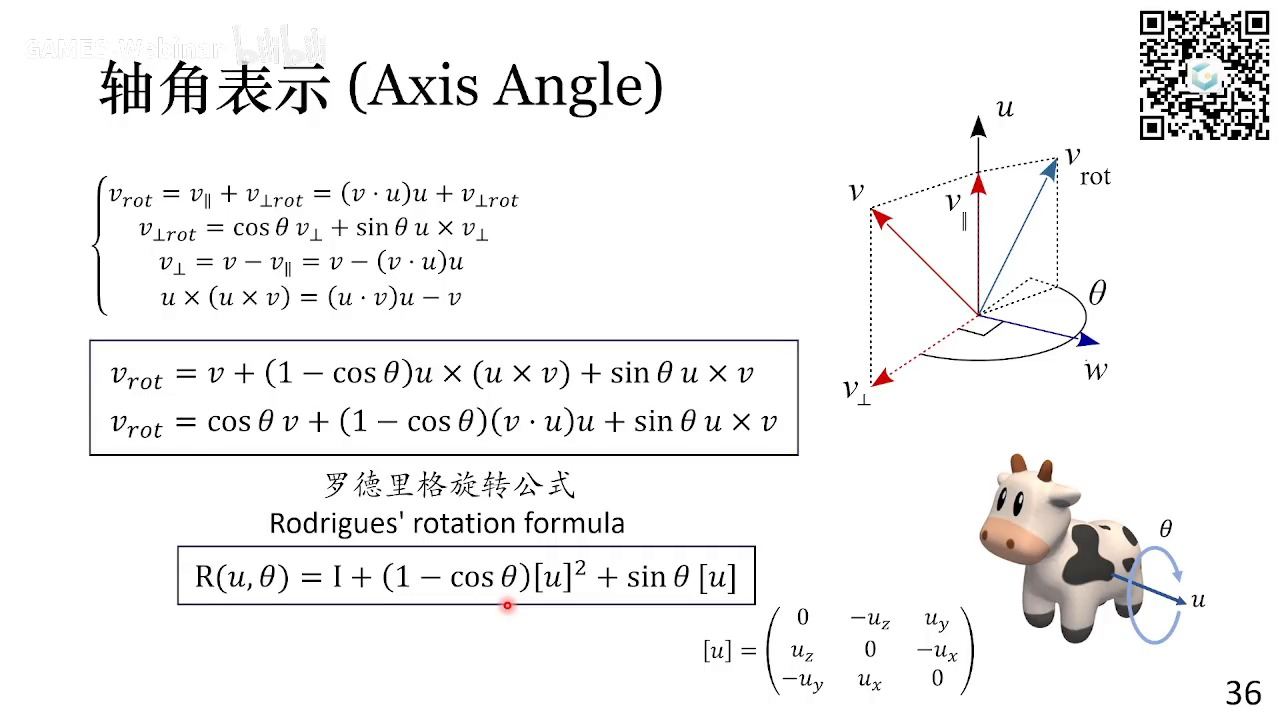
\includegraphics[width=0.92\textwidth]{figures/fig_23_axis_angle_derive.jpg}
\caption{轴角表示与罗德里格公式的推导：平行分量不变，垂直分量在平面内做二维旋转\vtag}
\end{figure}
\srcnote{00:48:15--00:48:30}
\end{minipage}


为了把公式写成矩阵形式，引入叉乘矩阵 $[\mathbf u]$，使 $[\mathbf u]\mathbf v=\mathbf u\times\mathbf v$：
\[
[\mathbf u]=\begin{pmatrix}0&-u_z&u_y\\u_z&0&-u_x\\-u_y&u_x&0\end{pmatrix},\qquad
\mathrm R(\mathbf u,\theta)=\mathrm I+(1-\cos\theta)[\mathbf u]^2+\sin\theta\,[\mathbf u] .
\]
讲者强调这个公式很重要，建议大家回去自己推一遍。

\subsection{从旋转矩阵反求轴角}

给定 $\mathrm R$，如何求出 $\theta$ 和 $\mathbf u$？先求迹。由二重叉积，
\[
[\mathbf u]^2\mathbf v=\mathbf u\times(\mathbf u\times\mathbf v)=(\mathbf u\cdot\mathbf v)\mathbf u-(\mathbf u\cdot\mathbf u)\mathbf v=(\mathbf u\mathbf u^{\mathsf T}-\mathrm I)\mathbf v,
\]
所以 $[\mathbf u]^2=\mathbf u\mathbf u^{\mathsf T}-\mathrm I$，其迹为 $1-3=-2$；而 $[\mathbf u]$ 的迹为零。于是
\[
\operatorname{tr}\mathrm R=\operatorname{tr}\mathrm I+(1-\cos\theta)\operatorname{tr}[\mathbf u]^2=3-2(1-\cos\theta)=1+2\cos\theta,\qquad
\theta=\arccos\frac{\operatorname{tr}\mathrm R-1}{2}.
\]
再求转轴。$[\mathbf u]$ 是反对称矩阵，但 $[\mathbf u]^2$ 和 $\mathrm I$ 都是对称矩阵，所以 $\mathrm R-\mathrm R^{\mathsf T}=2\sin\theta\,[\mathbf u]$，读出反对称部分的三个元素即可：
\[
\mathbf u=\frac{1}{2\sin\theta}\begin{pmatrix}\mathrm R_{21}-\mathrm R_{12}\\ \mathrm R_{02}-\mathrm R_{20}\\ \mathrm R_{10}-\mathrm R_{01}\end{pmatrix}.
\]

\noindent\begin{minipage}{\textwidth}
\begin{figure}[H]
\centering
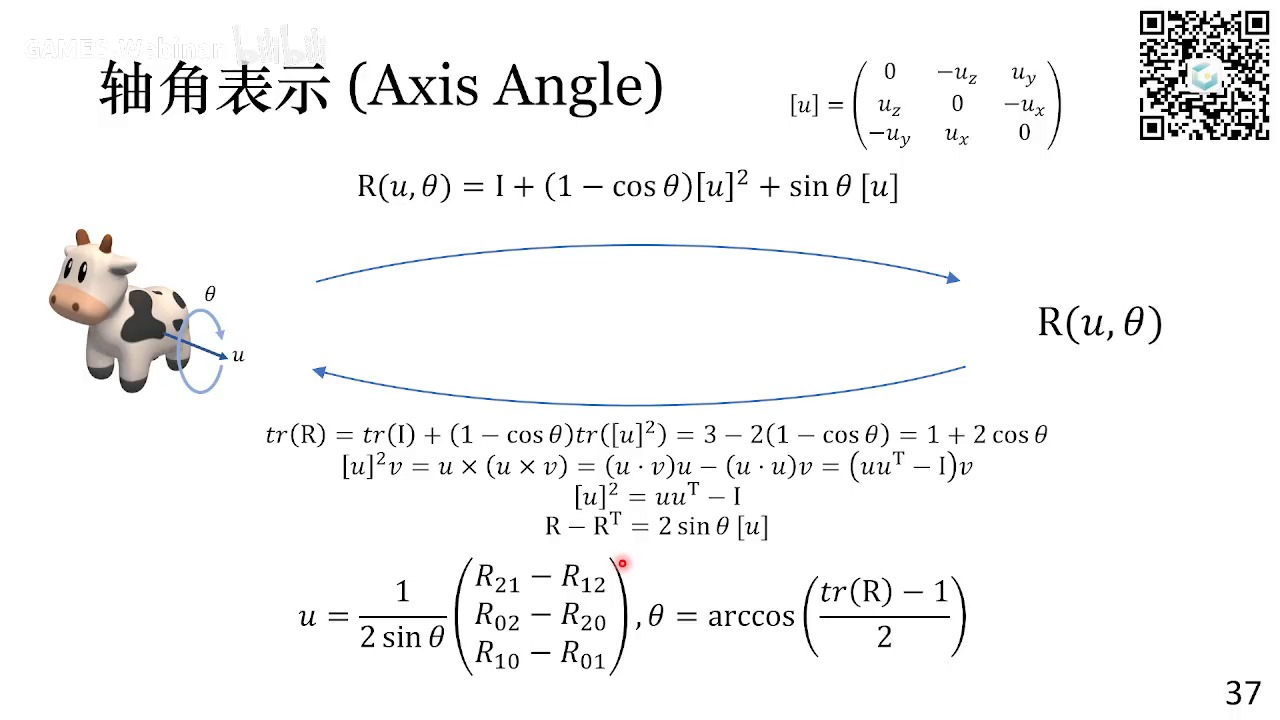
\includegraphics[width=0.92\textwidth]{figures/fig_24_axis_angle_inverse.jpg}
\caption{从旋转矩阵反求轴角：迹给出 $\theta$，反对称部分给出 $\mathbf u$\vtag}
\end{figure}
\srcnote{00:51:45--00:52:00}
\end{minipage}


\begin{warningbox}{$\theta$ 接近 $0$ 或 $\pi$ 时}
讲义作者补充：上式在 $\sin\theta\approx0$ 时分母趋零。$\theta\approx0$ 时旋转接近单位阵，转轴本身就不重要；$\theta\approx\pi$ 时 $\mathrm R-\mathrm R^{\mathsf T}\approx0$，转轴应改由对称部分 $\mathrm R+\mathrm I=2\mathbf u\mathbf u^{\mathsf T}$ 的某一非零列归一化得到。实际库函数都会对这两种情况单独处理。
\end{warningbox}

\subsection{指数形式与李代数}

罗德里格公式还可以写成矩阵指数：
\[
\mathrm R(\mathbf u,\theta)=\exp(\theta[\mathbf u])=\exp([\boldsymbol\theta]) .
\]
验证方法是把指数按泰勒级数展开 $\exp(\theta[\mathbf u])=\mathrm I+\theta[\mathbf u]+\frac1{2!}\theta^2[\mathbf u]^2+\frac1{3!}\theta^3[\mathbf u]^3+\cdots$，并利用 $[\mathbf u]$ 的幂的周期性：
\[
[\mathbf u]^2=\mathbf u\mathbf u^{\mathsf T}-\mathrm I,\quad
[\mathbf u]^3=-[\mathbf u],\quad
[\mathbf u]^4=-[\mathbf u]^2,\quad
[\mathbf u]^5=[\mathbf u],\ \dots
\]
把奇次项和偶次项分别合并：
\[
\exp(\theta[\mathbf u])=\mathrm I+\Big(\theta-\tfrac1{3!}\theta^3+\tfrac1{5!}\theta^5-\cdots\Big)[\mathbf u]+\Big(\tfrac1{2!}\theta^2-\tfrac1{4!}\theta^4+\cdots\Big)[\mathbf u]^2
=\mathrm I+\sin\theta\,[\mathbf u]+(1-\cos\theta)[\mathbf u]^2 .
\]
系数正好是 $\sin\theta$ 和 $1-\cos\theta$ 的泰勒级数，结果与罗德里格公式一致。

\noindent\begin{minipage}{\textwidth}
\begin{figure}[H]
\centering
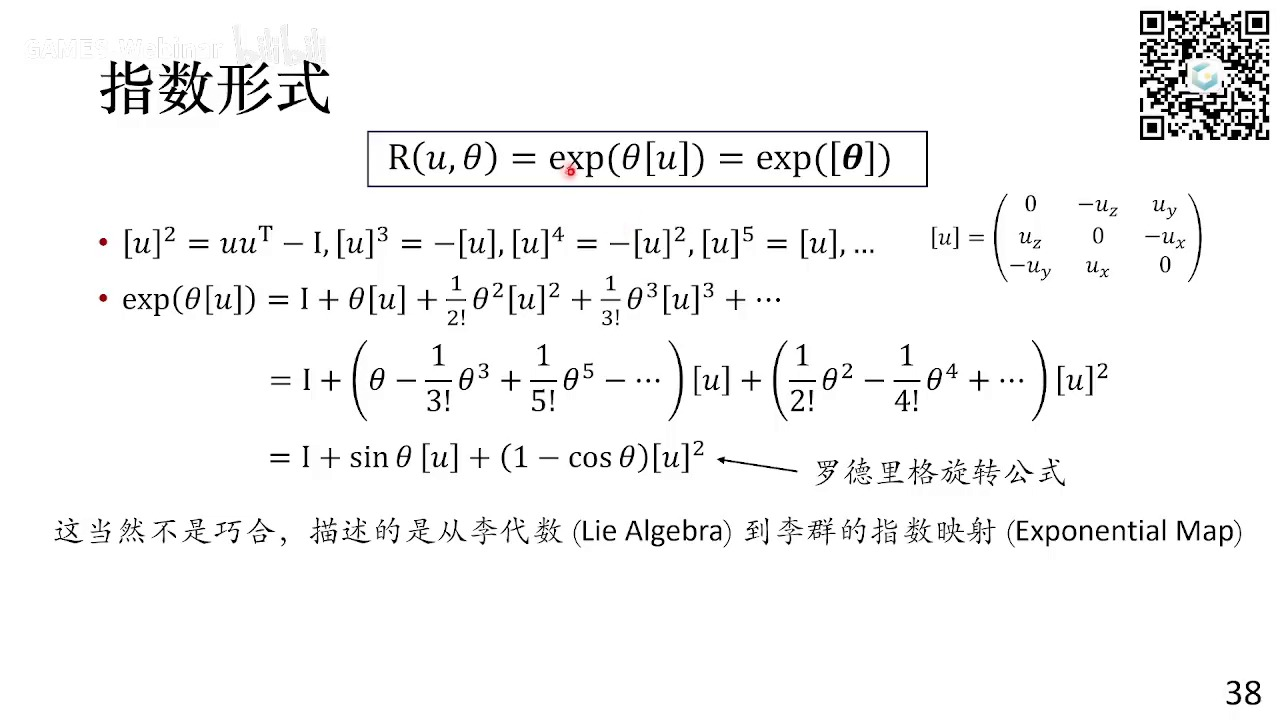
\includegraphics[width=0.92\textwidth]{figures/fig_25_exp_form.jpg}
\caption{指数形式：泰勒展开后合并奇偶项，恰好得到罗德里格公式\vtag}
\end{figure}
\srcnote{00:55:15--00:55:30}
\end{minipage}


讲者说这当然不是巧合：它描述的是从\textbf{李代数}（Lie algebra）到李群的\textbf{指数映射}（exponential map）。直观地说，从单位旋转出发，在切空间里沿方向 $[\boldsymbol\theta]$ 走，指数映射把这一步“卷”到旋转流形上，就像在球面上沿着切线方向一直往前走，实际走的是一条大圆弧。

\subsection{轴角插值}

轴角表示可以用来做\textbf{相对旋转插值}。先求从 $\mathrm R_0$ 到 $\mathrm R_1$ 的相对旋转 $\Delta\mathrm R=\mathrm R_1\mathrm R_0^{\mathsf T}$，把它转换成轴角 $(\Delta\theta,\Delta\mathbf u)$；然后只对角度做线性插值，转轴保持不变：
\[
\theta_t=t\,\Delta\theta,\qquad \Delta\mathrm R_t\leftarrow(\theta_t,\Delta\mathbf u),\qquad \mathrm R(t)=\Delta\mathrm R_t\,\mathrm R_0 .
\]
这样得到的中间旋转在 $t=0,0.2,0.5,0.8,1$ 时都是合法的旋转，并且是绕固定轴匀速转过去的。

\noindent\begin{minipage}{\textwidth}
\begin{figure}[H]
\centering
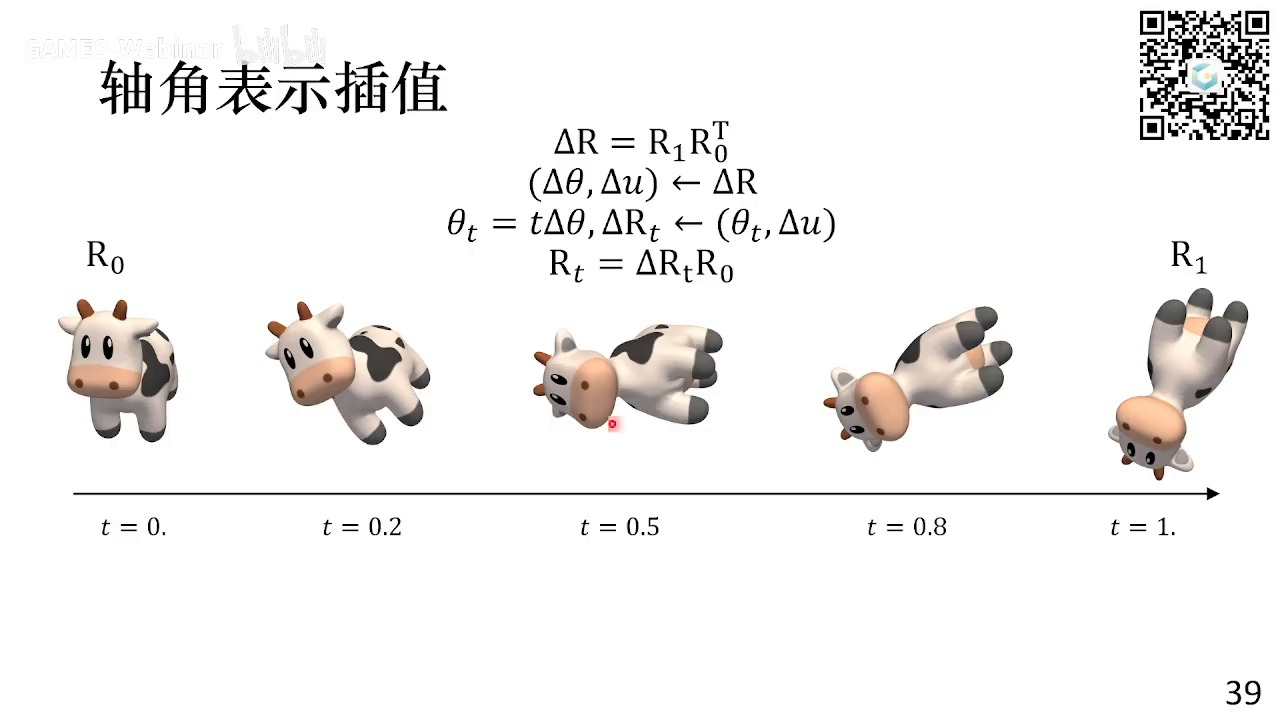
\includegraphics[width=0.92\textwidth]{figures/fig_26_axis_angle_interp.jpg}
\caption{轴角插值：对相对旋转的角度线性插值\vtag}
\end{figure}
\srcnote{00:56:45--00:57:00}
\end{minipage}


\begin{warningbox}{不要直接插值旋转向量}
直接对两个旋转向量做线性插值 $\boldsymbol\theta_t=(1-t)\boldsymbol\theta_0+t\boldsymbol\theta_1$，结果是不对的。课件中的例子是 $\boldsymbol\theta_0=\frac{3\pi}2(1,0,0)$，$\boldsymbol\theta_1=\frac{3\pi}2(0,1,0)$：线性插值的中间结果绕了很大的弯（$\times$），而相对旋转插值得到了正确的结果（$\checkmark$）。原因是旋转向量所在的 $\mathbb R^3$ 并不是旋转流形本身，两点间的直线不对应流形上的最短路径。
\end{warningbox}

\noindent\begin{minipage}{\textwidth}
\begin{figure}[H]
\centering
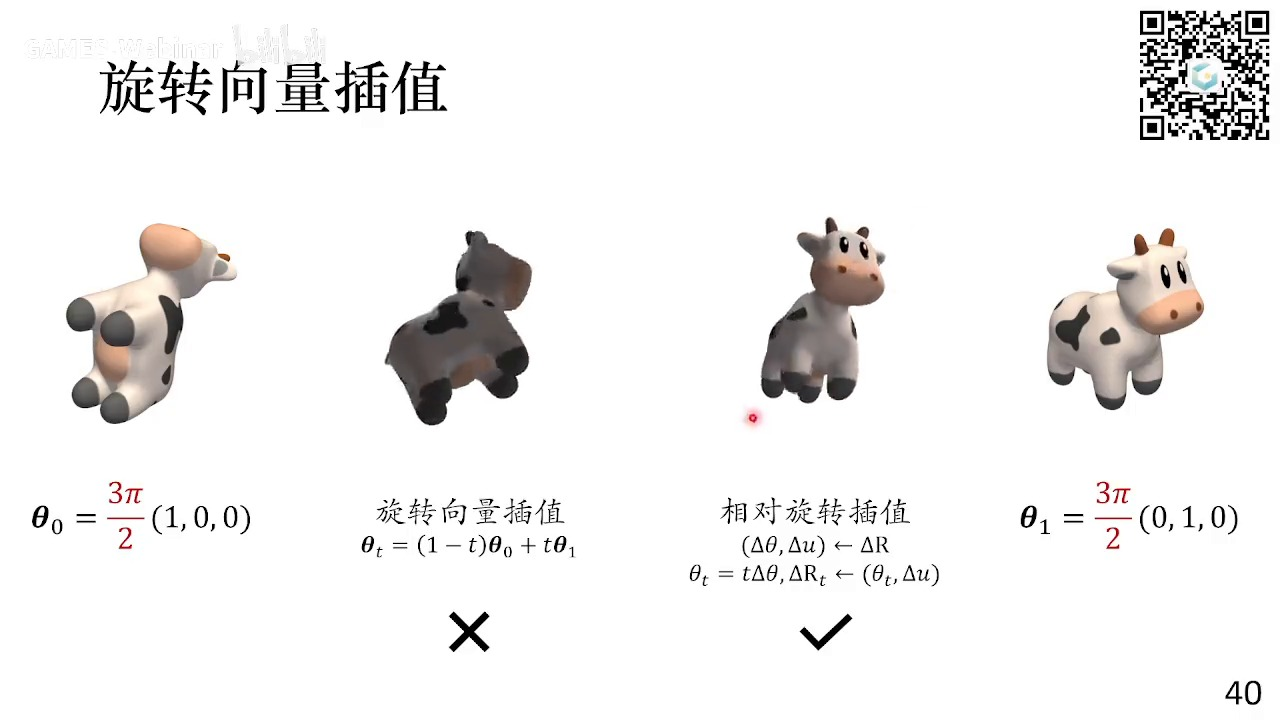
\includegraphics[width=0.92\textwidth]{figures/fig_27_rotvec_interp.jpg}
\caption{旋转向量直接线性插值（$\times$）与相对旋转插值（$\checkmark$）的对比\vtag}
\end{figure}
\srcnote{00:57:45--00:58:00}
\end{minipage}


\section{四元数}

\subsection{从复数与二维旋转说起}

四元数（quaternion）由哈密顿（William Rowan Hamilton）发明。讲者讲了一个小故事：哈密顿一直在想，用什么样的数据结构来表达三维旋转。某一天他走到都柏林的一座桥边，突然想通了，就把公式刻在了桥上。那块石碑至今还在桥边，上面刻的就是 $i^2=j^2=k^2=ijk=-1$。

\noindent\begin{minipage}{\textwidth}
\begin{figure}[H]
\centering
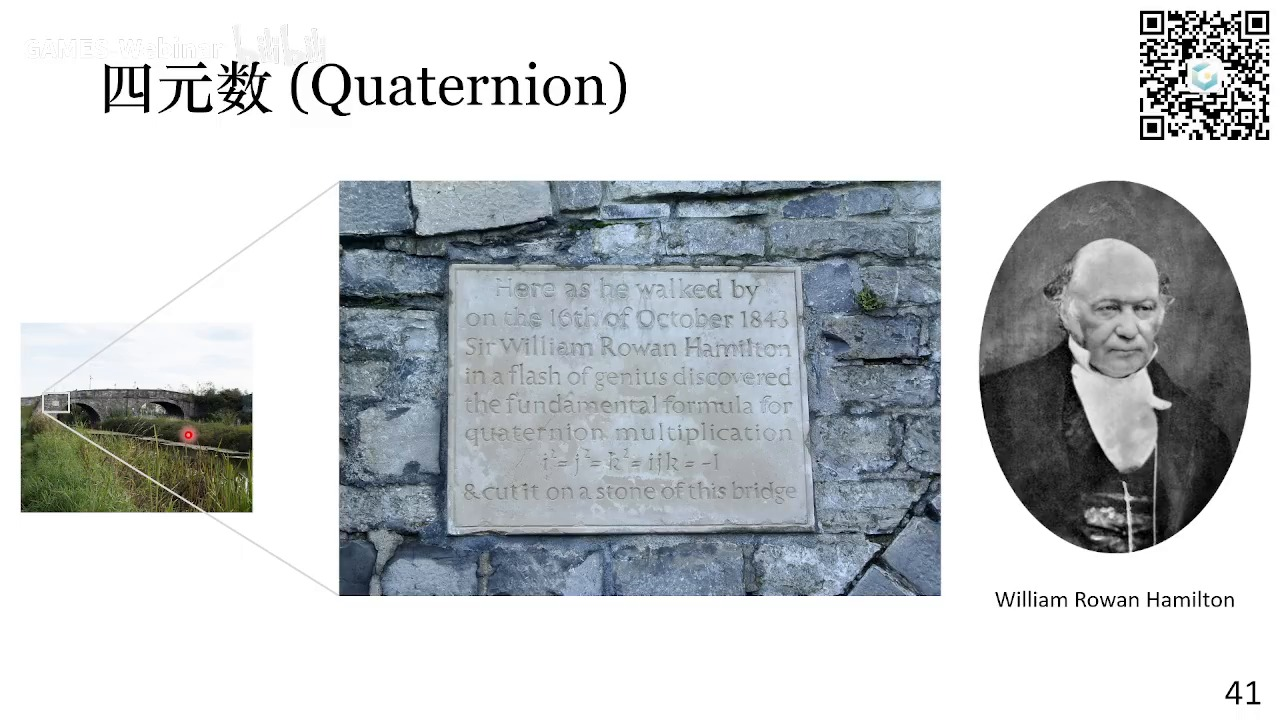
\includegraphics[width=0.92\textwidth]{figures/fig_28_hamilton.jpg}
\caption{四元数的发明者哈密顿，以及刻在桥上的四元数公式\vtag}
\end{figure}
\srcnote{00:59:45--01:00:00}
\end{minipage}


在介绍四元数之前，先从二维旋转入手。二维旋转可以写成矩阵，也可以写成复数。设 $c=a+ib$，$z=x+iy$，则
\[
cz=(ax-by)+i(bx+ay),\qquad
\begin{pmatrix}ax-by\\bx+ay\end{pmatrix}=\begin{pmatrix}a&-b\\b&a\end{pmatrix}\begin{pmatrix}x\\y\end{pmatrix}.
\]
所以复数 $c$ 可以看成矩阵 $[c]=\begin{pmatrix}a&-b\\b&a\end{pmatrix}$。特别地，虚数单位对应 $[i]=\begin{pmatrix}0&-1\\1&0\end{pmatrix}$，它的幂依次是 $-\mathrm I$、$-[i]$、$\mathrm I$，与 $i^2=-1$、$i^3=-i$、$i^4=1$ 完全对应。于是
\[
\exp(\theta[i])=\sum_k\frac1{k!}\theta^k[i]^k=\cos\theta\,\mathrm I+\sin\theta\,[i]
=\begin{pmatrix}\cos\theta&-\sin\theta\\ \sin\theta&\cos\theta\end{pmatrix},
\]
对应的复数形式就是欧拉公式 $e^{i\theta}=\cos\theta+i\sin\theta$，二维旋转即 $z'=(\cos\theta+i\sin\theta)z$。

\noindent\begin{minipage}{\textwidth}
\begin{figure}[H]
\centering
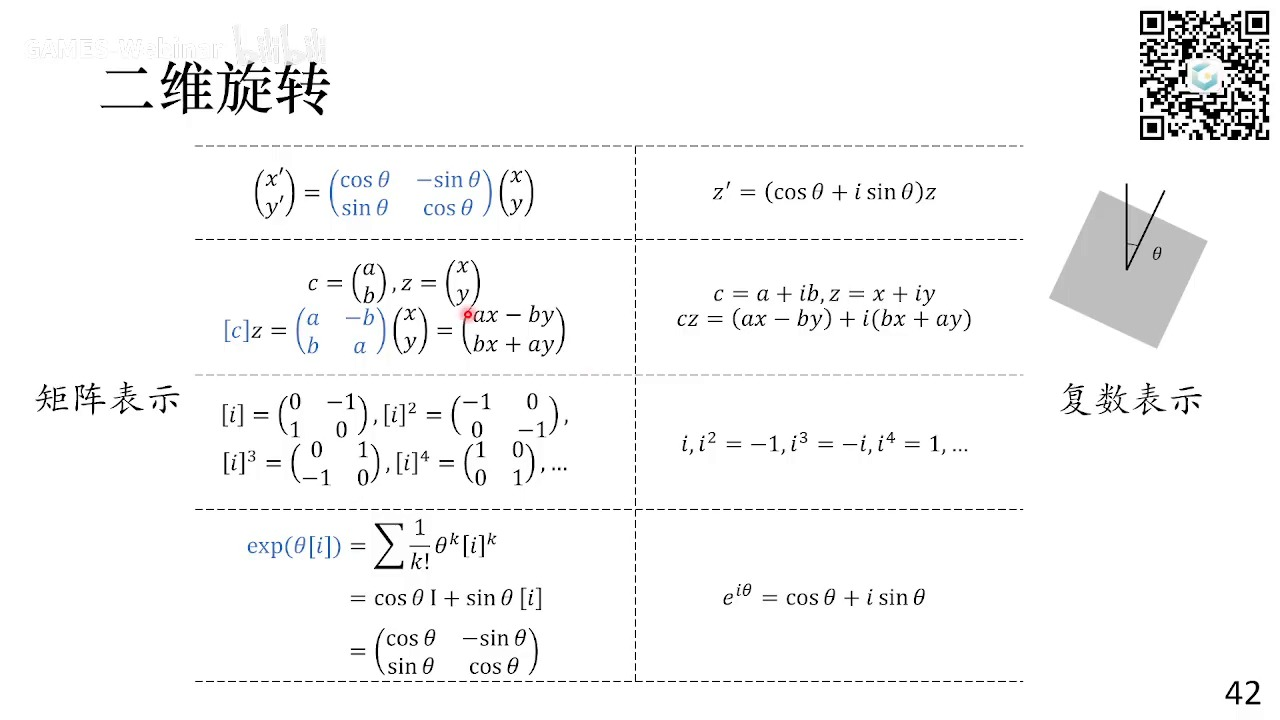
\includegraphics[width=0.92\textwidth]{figures/fig_29_complex2d.jpg}
\caption{二维旋转的矩阵表示与复数表示：$[i]$ 的幂与 $i$ 的幂一一对应\vtag}
\end{figure}
\srcnote{01:04:15--01:04:30}
\end{minipage}


\subsection{四元数的乘法与 Graßmann 积}

三维旋转的矩阵表示是 $\mathrm R(\mathbf u,\theta)=\exp(\theta[\mathbf u])$，与二维的 $\exp(\theta[i])$ 形式相同。类比复数，四元数写成
\[
q=a+bi+cj+dk,\qquad i^2=j^2=k^2=ijk=-1 .
\]
两个四元数相乘，把 8 个系数逐项展开，并查乘法表（如 $ij=k$，$ji=-k$）：
\[
\begin{aligned}
q_1q_2&=(a+bi+cj+dk)(e+fi+gj+hk)\\
&=(ae-bf-cg-dh)+(be+af-dg+ch)i+(ce+df+ag-bh)j+(de-cf+bg+ah)k .
\end{aligned}
\]
它也可以写成矩阵乘向量的形式：
\[
q_1q_2=\begin{pmatrix}a&-b&-c&-d\\b&a&-d&c\\c&d&a&-b\\d&-c&b&a\end{pmatrix}\begin{pmatrix}e\\f\\g\\h\end{pmatrix}.
\]

\noindent\begin{minipage}{\textwidth}
\begin{figure}[H]
\centering
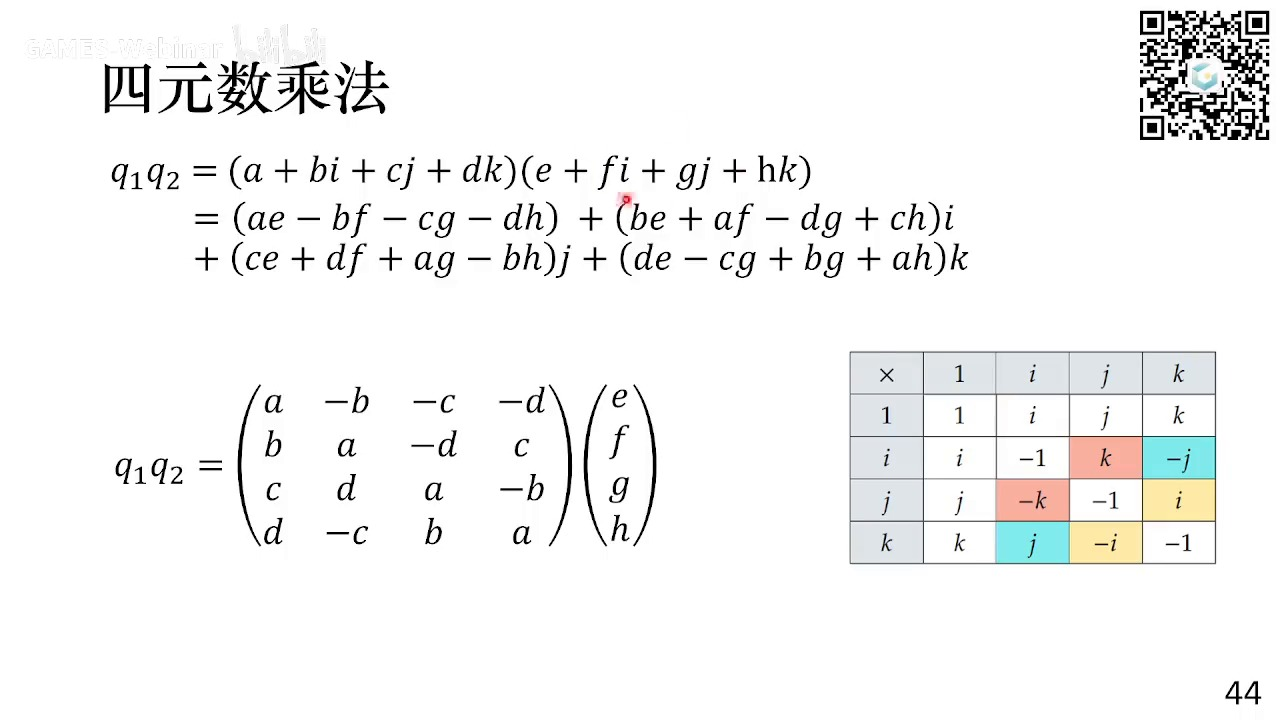
\includegraphics[width=0.92\textwidth]{figures/fig_30_quat_mult.jpg}
\caption{四元数乘法：逐项展开与乘法表，以及等价的矩阵形式\vtag}
\end{figure}
\srcnote{01:09:15--01:09:30}
\end{minipage}


把四元数写成“标量 $+$ 向量”的形式更清楚：$q_1=(a,\mathbf v)$，$\mathbf v=bi+cj+dk$；$q_2=(e,\mathbf u)$，$\mathbf u=fi+gj+hk$。上面的乘积整理后得到 \textbf{Graßmann 积}：
\[
q_1q_2=(ae-\mathbf v\cdot\mathbf u,\ a\mathbf u+e\mathbf v+\mathbf v\times\mathbf u) .
\]
因为叉积不可交换，$q_1q_2\neq q_2q_1$。如果 $a=e=0$，称为纯四元数，此时 $q_1q_2=(-\mathbf v\cdot\mathbf u,\ \mathbf v\times\mathbf u)$，同时包含了点乘和叉乘。对应的矩阵形式是
\[
q_1q_2=\begin{pmatrix}a&-\mathbf v^{\mathsf T}\\ \mathbf v&a\mathrm I+[\mathbf v]\end{pmatrix}\begin{pmatrix}e\\ \mathbf u\end{pmatrix}.
\]
讲者指出，旋转矩阵里有叉乘，四元数乘法里也有叉乘，这正是四元数能和旋转建立联系的原因。

\noindent\begin{minipage}{\textwidth}
\begin{figure}[H]
\centering
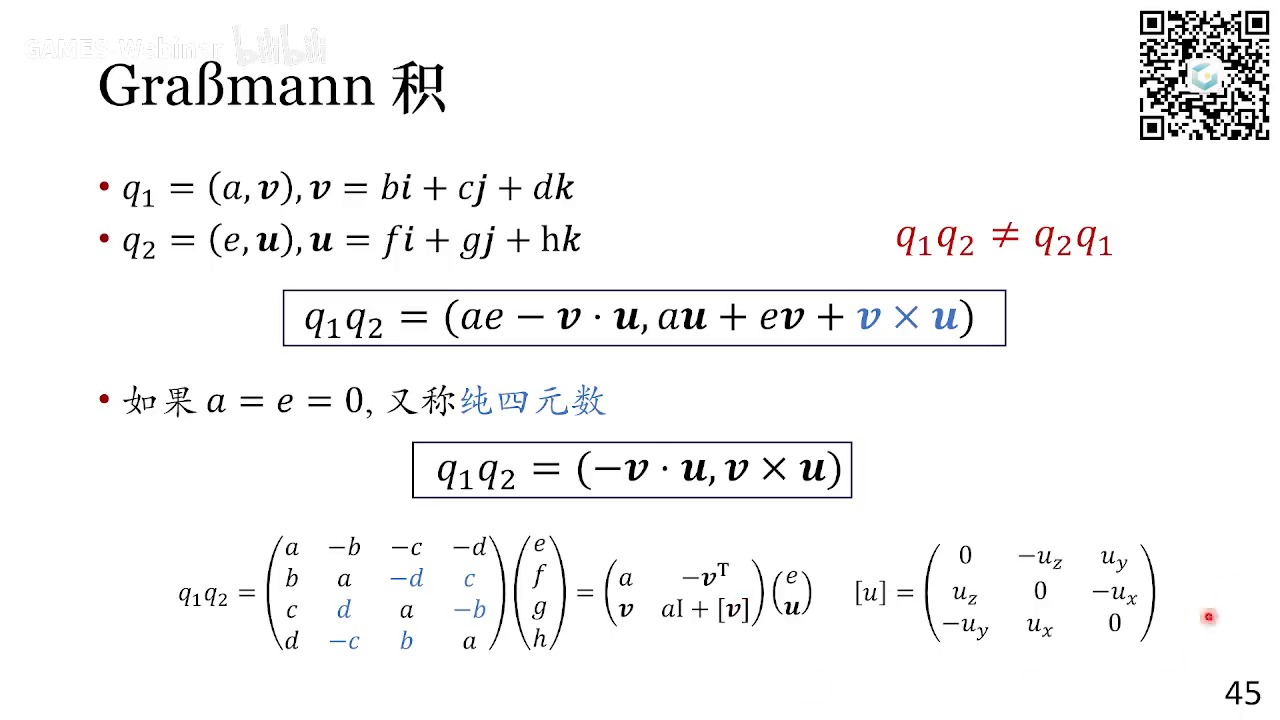
\includegraphics[width=0.92\textwidth]{figures/fig_31_grassmann.jpg}
\caption{Graßmann 积：$q_1q_2=(ae-\mathbf v\cdot\mathbf u,\ a\mathbf u+e\mathbf v+\mathbf v\times\mathbf u)$\vtag}
\end{figure}
\srcnote{01:11:30--01:11:45}
\end{minipage}


\subsection{共轭、模长与逆}

四元数的共轭像复数一样，把虚部取负：$q^*=a-bi-cj-dk=(a,-\mathbf v)$。于是
\[
qq^*=a^2+b^2+c^2+d^2=\|q\|^2=(a^2+\mathbf v\cdot\mathbf v,\ \mathbf 0),
\]
向量部分 $-a\mathbf v+a\mathbf v-\mathbf v\times\mathbf v$ 正好抵消为零。由此得到逆
\[
q^{-1}=\frac{q^*}{\|q\|^2}.
\]
对于单位四元数（unit quaternion），$\|q\|=1$，有 $q^{-1}=q^*$。

\noindent\begin{minipage}{\textwidth}
\begin{figure}[H]
\centering
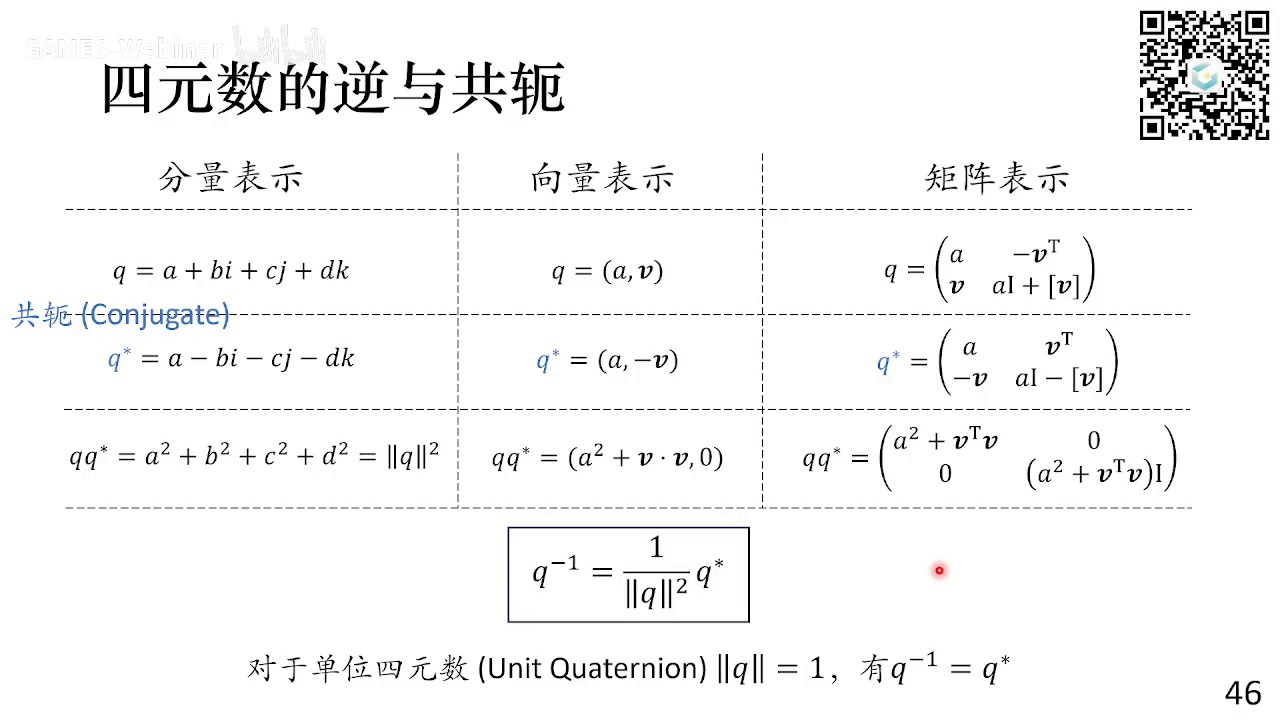
\includegraphics[width=0.92\textwidth]{figures/fig_32_quat_inverse.jpg}
\caption{四元数的共轭与逆：分量、向量与矩阵三种表示\vtag}
\end{figure}
\srcnote{01:15:30--01:15:45}
\end{minipage}


\subsection{四元数如何表示旋转}

把三维向量 $\mathbf v$ 写成实部为零的纯虚四元数 $v=(0,\mathbf v)$。先试试取 $q=(\cos\theta,\ \sin\theta\,\mathbf u)$ 直接左乘：
\[
qv=(-\sin\theta\,\mathbf u\cdot\mathbf v,\ \cos\theta\,\mathbf v+\sin\theta\,\mathbf u\times\mathbf v).
\]
对比罗德里格公式，它看起来接近旋转变换，但少了 $(1-\cos\theta)(\mathbf v\cdot\mathbf u)\mathbf u$ 一项，并且实部不为零。

\noindent\begin{minipage}{\textwidth}
\begin{figure}[H]
\centering
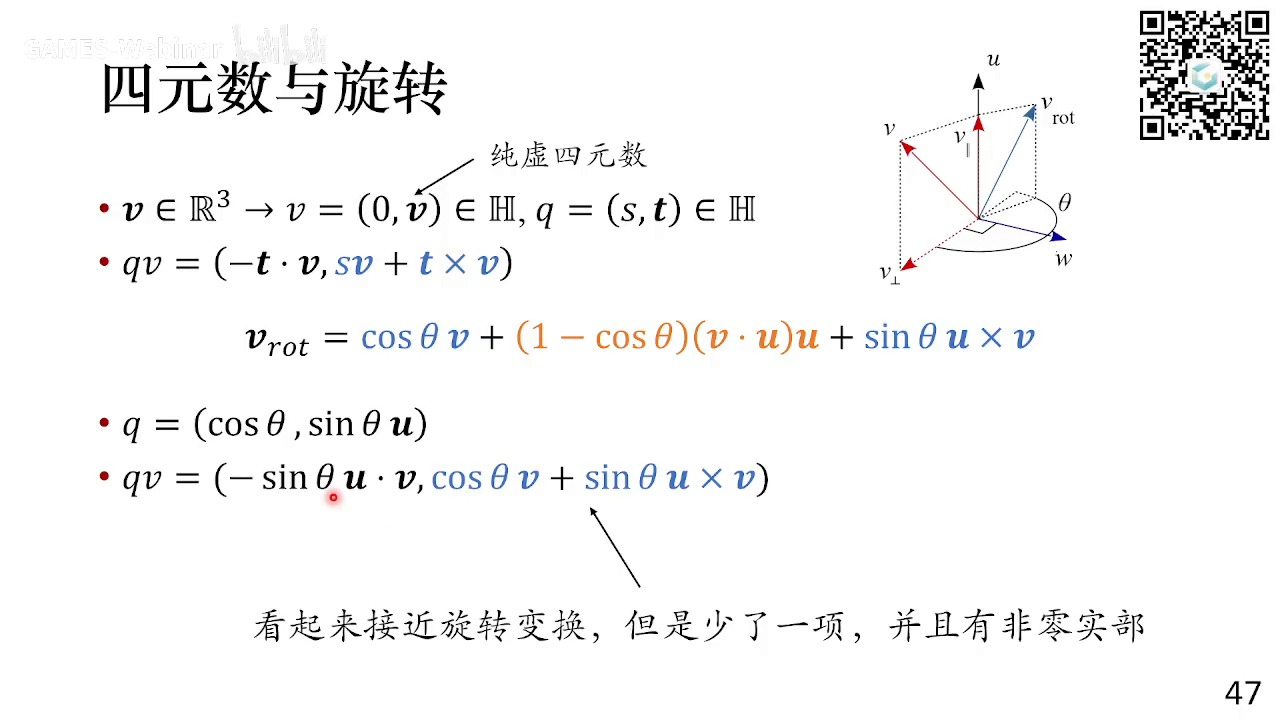
\includegraphics[width=0.92\textwidth]{figures/fig_33_quat_rotation_try.jpg}
\caption{只左乘 $q$：接近旋转，但少一项且有非零实部\vtag}
\end{figure}
\srcnote{01:17:30--01:17:45}
\end{minipage}


改为“两边夹”：$q$ 是单位四元数，$q^{-1}=q^*=(c,-s\mathbf u)$，其中 $c=\cos\theta$，$s=\sin\theta$。用 Graßmann 积展开
\[
qvq^{-1}=(c,s\mathbf u)(0,\mathbf v)(c,-s\mathbf u)
=\big(0,\ (c^2-s^2)\mathbf v+2sc\,\mathbf u\times\mathbf v+2s^2(\mathbf u\cdot\mathbf v)\mathbf u\big),
\]
实部恰好抵消为零。利用倍角公式 $c^2-s^2=\cos2\theta$，$2sc=\sin2\theta$，$2s^2=1-\cos2\theta$，这正是绕 $\mathbf u$ 旋转 $2\theta$ 的罗德里格公式。所以要旋转 $\theta$，应取半角：
\[
q=\Big(\cos\frac\theta2,\ \sin\frac\theta2\,\mathbf u\Big),\qquad v_{\mathrm{rot}}=qvq^* .
\]

\noindent\begin{minipage}{\textwidth}
\begin{figure}[H]
\centering
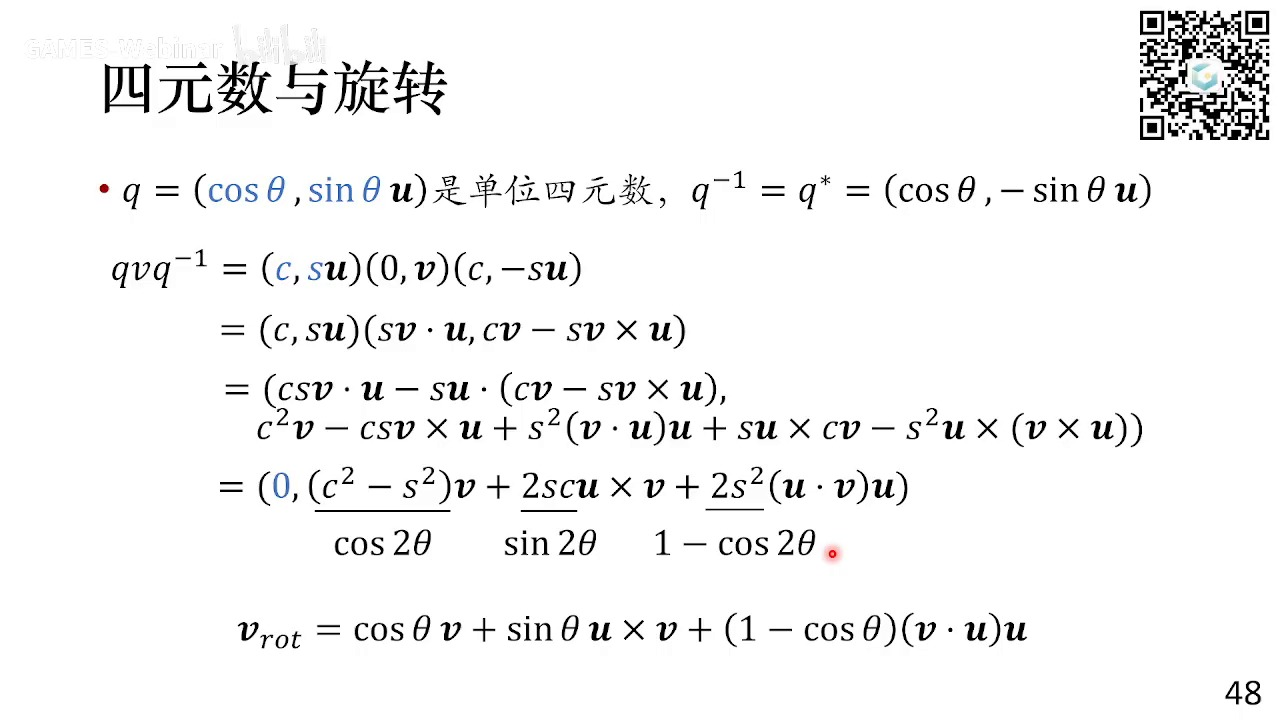
\includegraphics[width=0.92\textwidth]{figures/fig_34_quat_rotation.jpg}
\caption{$qvq^{-1}$ 的展开：实部消失，向量部分是转角 $2\theta$ 的罗德里格公式，故取半角\vtag}
\end{figure}
\srcnote{01:20:45--01:21:00}
\end{minipage}


\begin{knowledgebox}{为什么是 4 个数、为什么是半角}
讲者推荐了两份直观的材料来回答“为什么需要 4 自由度的四元数表示旋转”和“为什么是两次半角相乘”：3Blue1Brown 的四元数可视化视频（B 站 BV1SW411y7W1），以及 Krasjet 的《四元数与三维旋转》讲义（krasjet.github.io/quaternion）。约束 $\|q\|=1$ 去掉了一个自由度，所以单位四元数的自由度仍是 3；讲者在弹幕答疑时也确认了这一点：$q$ 虽然有四个分量，但限制它为单位四元数相当于加了一个约束；半角来自“左乘一次、右乘一次”，两次各转半角，合起来转一整个角度。
\end{knowledgebox}

\subsection{四元数旋转的性质}

\begin{itemize}
\item \textbf{多次旋转}：先 $q_1$ 再 $q_2$，有 $v_1=q_1vq_1^*$，$v_2=q_2v_1q_2^*=(q_2q_1)v(q_2q_1)^*$，所以复合旋转就是四元数相乘 $q=q_nq_{n-1}\cdots q_1$。这里用到了共轭的性质 $q_1^*q_2^*=(q_2q_1)^*$，与矩阵转置 $(\mathrm A\mathrm B)^{\mathsf T}=\mathrm B^{\mathsf T}\mathrm A^{\mathsf T}$ 的规则一样，顺序要反过来。
\item \textbf{双重覆盖}：$q$ 与 $-q$ 表示相同的旋转，因为 $(-q)v(-q)^*=qvq^*$，两个负号相乘为正。
\item \textbf{指数形式}：$q=\big(\cos\frac\theta2,\sin\frac\theta2\mathbf u\big)=\exp\big(\frac\theta2u\big)$，其中 $u=(0,\mathbf u)$，于是
\[
v_{\mathrm{rot}}=\exp\Big(\frac\theta2u\Big)\,v\,\exp\Big(-\frac\theta2u\Big).
\]
讲者说这个指数形式只是给大家看看，实际计算还是要回到 Graßmann 积的公式。
\end{itemize}

\noindent\begin{minipage}{\textwidth}
\begin{figure}[H]
\centering
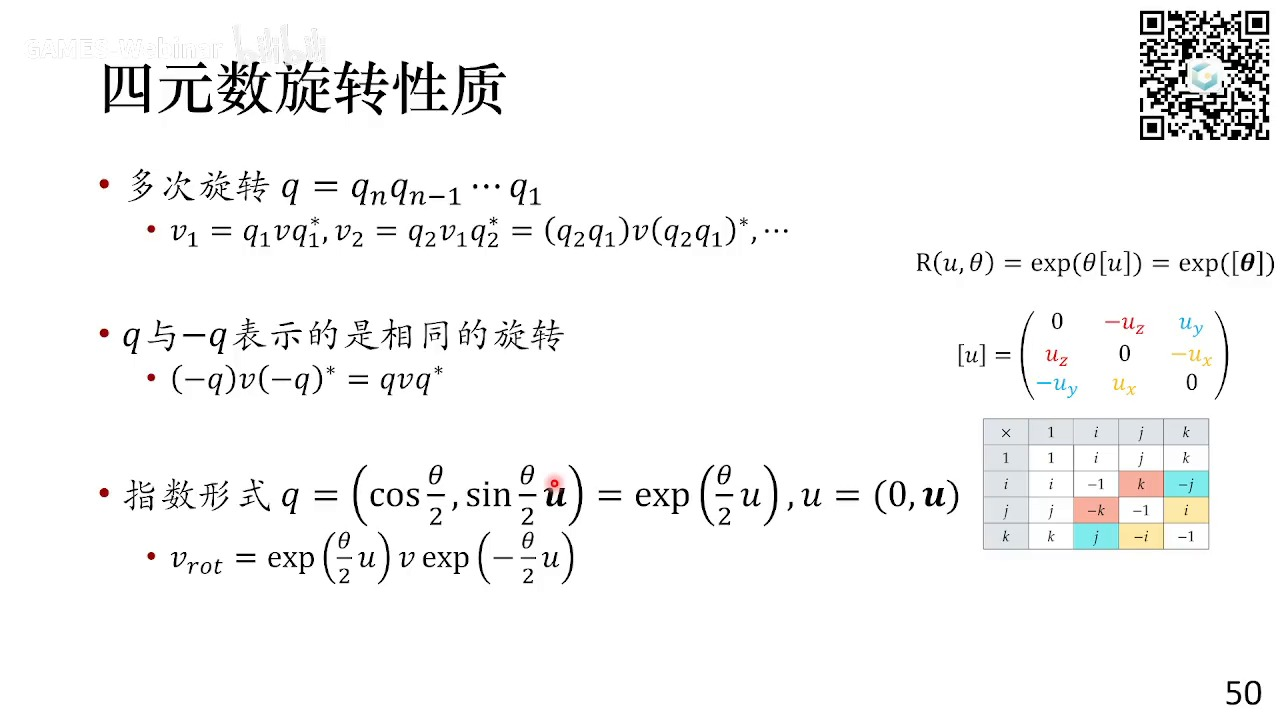
\includegraphics[width=0.92\textwidth]{figures/fig_35_quat_properties.jpg}
\caption{四元数旋转的性质：复合即相乘，$q$ 与 $-q$ 等价，指数形式\vtag}
\end{figure}
\srcnote{01:26:00--01:26:15}
\end{minipage}


\section{四元数插值}

\subsection{四元数旋转流形}

单位四元数满足 $\|q\|=1$，在四维空间 $\mathbb H$ 中构成一个球面（三维球面）。所以用四元数观察旋转，旋转流形就是四维空间中的三维球面，插值问题变成在这个球面上从 $q_0$ 走到 $q_1$。

\noindent\begin{minipage}{\textwidth}
\begin{figure}[H]
\centering
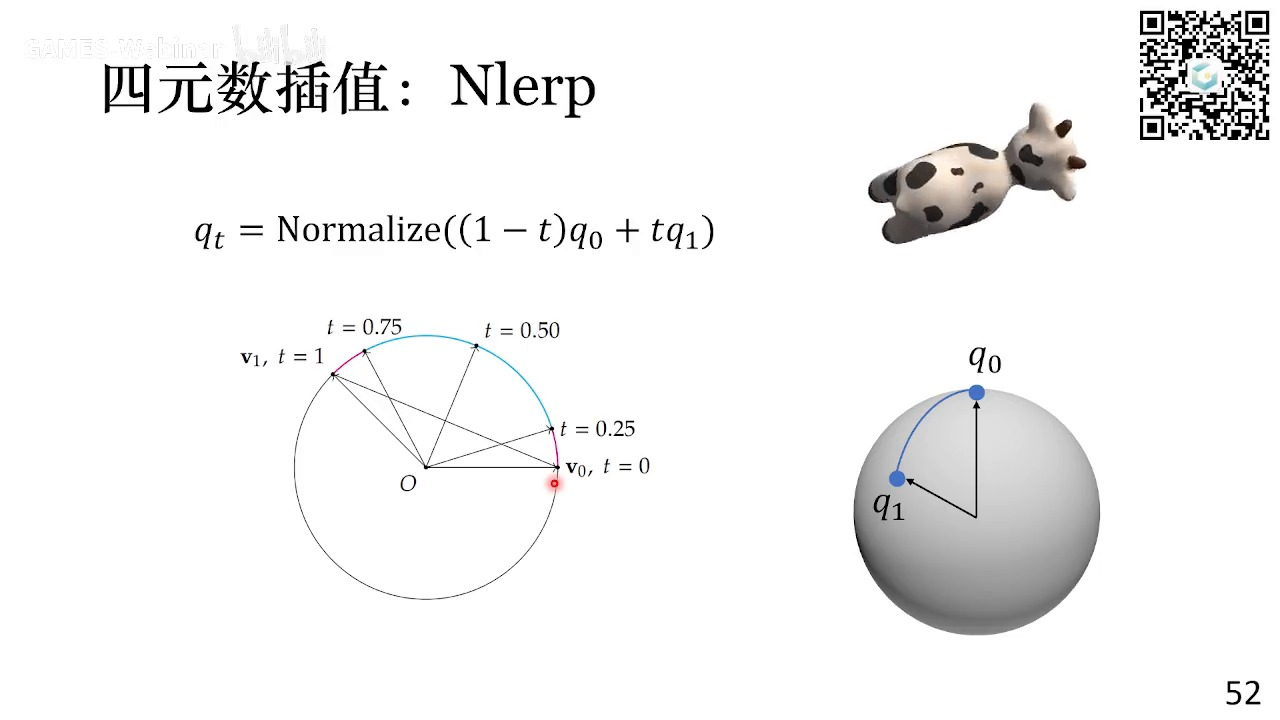
\includegraphics[width=0.92\textwidth]{figures/fig_36_quat_manifold.jpg}
\caption{四元数表示的旋转流形：四维空间中的单位球面\vtag}
\end{figure}
\srcnote{01:27:30--01:27:45}
\end{minipage}


\subsection{Nlerp}

最简单的做法是先线性插值，再归一化，拉回球面：
\[
q_t=\mathrm{Normalize}\big((1-t)q_0+tq_1\big) .
\]
这称为 Nlerp。它的结果总是合法的旋转，但有一个明显的问题：取 $t=0.25,0.5,0.75$ 的四等分点观察，弦上等距的点投影到圆弧上并不等距，中间稀、两头密，于是旋转先慢、再快、再慢，有明显的加速减速过程。

\noindent\begin{minipage}{\textwidth}
\begin{figure}[H]
\centering
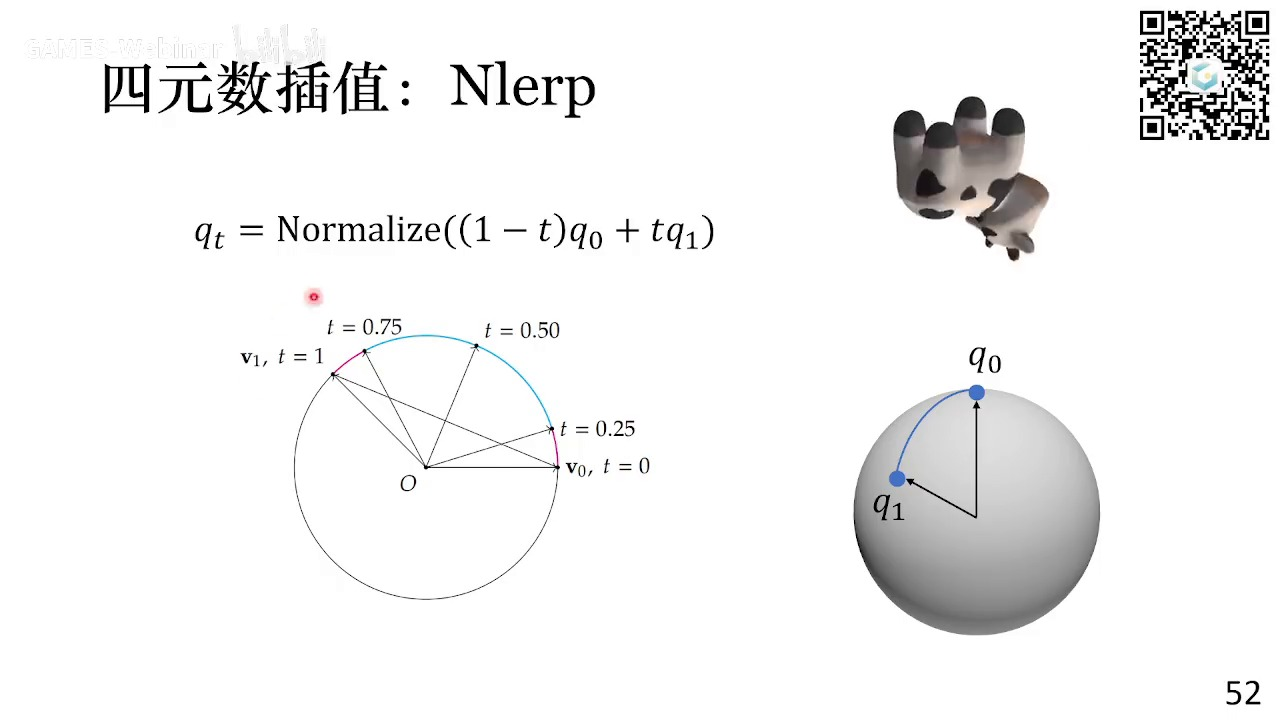
\includegraphics[width=0.92\textwidth]{figures/fig_37_nlerp.jpg}
\caption{Nlerp：线性插值后归一化，弦上等距的点在弧上不等距\vtag}
\end{figure}
\srcnote{01:29:15--01:29:30}
\end{minipage}


\subsection{四元数夹角与旋转角度}

两个四元数在球面上的夹角和它们之间的旋转角度是什么关系？取 $q_0=(1,\mathbf 0)$，即不旋转，以及 $q_1=\big(\cos\frac\theta2,\sin\frac\theta2\mathbf u\big)$，即绕 $\mathbf u$ 转 $\theta$。用点乘公式，
\[
\cos\varphi=\frac{\langle q_0,q_1\rangle}{\|q_0\|\,\|q_1\|}=\cos\frac\theta2
\;\Longrightarrow\;
\varphi=\frac12\theta .
\]
四元数之间的夹角是实际旋转角度的一半。

\noindent\begin{minipage}{\textwidth}
\begin{figure}[H]
\centering
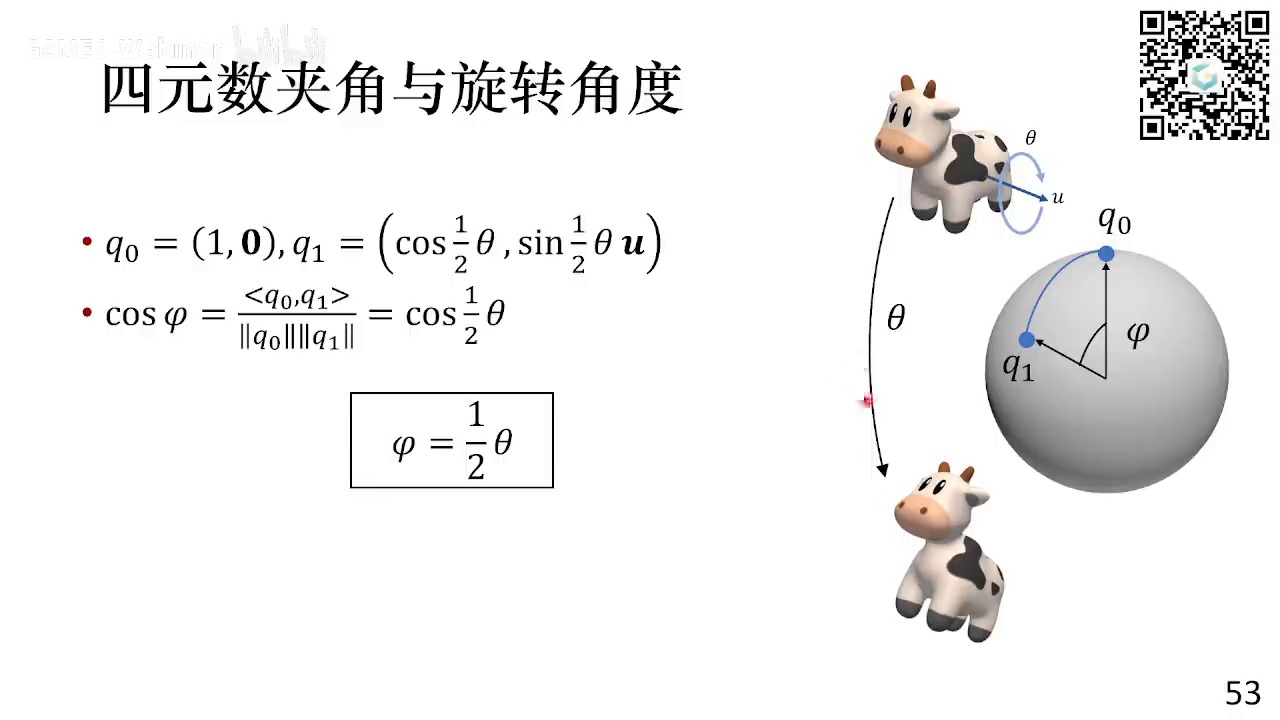
\includegraphics[width=0.92\textwidth]{figures/fig_38_quat_angle.jpg}
\caption{四元数夹角 $\varphi$ 等于旋转角度 $\theta$ 的一半\vtag}
\end{figure}
\srcnote{01:30:45--01:31:00}
\end{minipage}


\subsection{Slerp}

要匀速转动，就要沿大圆弧按角度等分。球面线性插值（Slerp）为
\[
q_t=\frac{\sin\big((1-t)\theta\big)}{\sin\theta}\,q_0+\frac{\sin(t\theta)}{\sin\theta}\,q_1,\qquad
\theta=\arccos\langle q_0,q_1\rangle ,
\]
这里的 $\theta$ 是两个四元数之间的夹角。Slerp 的结果比 Nlerp 好很多，奶牛是匀速转过去的。代价是计算更慢：Slerp 需要算三角函数，Nlerp 只需要做一次线性插值和一次归一化。

\noindent\begin{minipage}{\textwidth}
\begin{figure}[H]
\centering
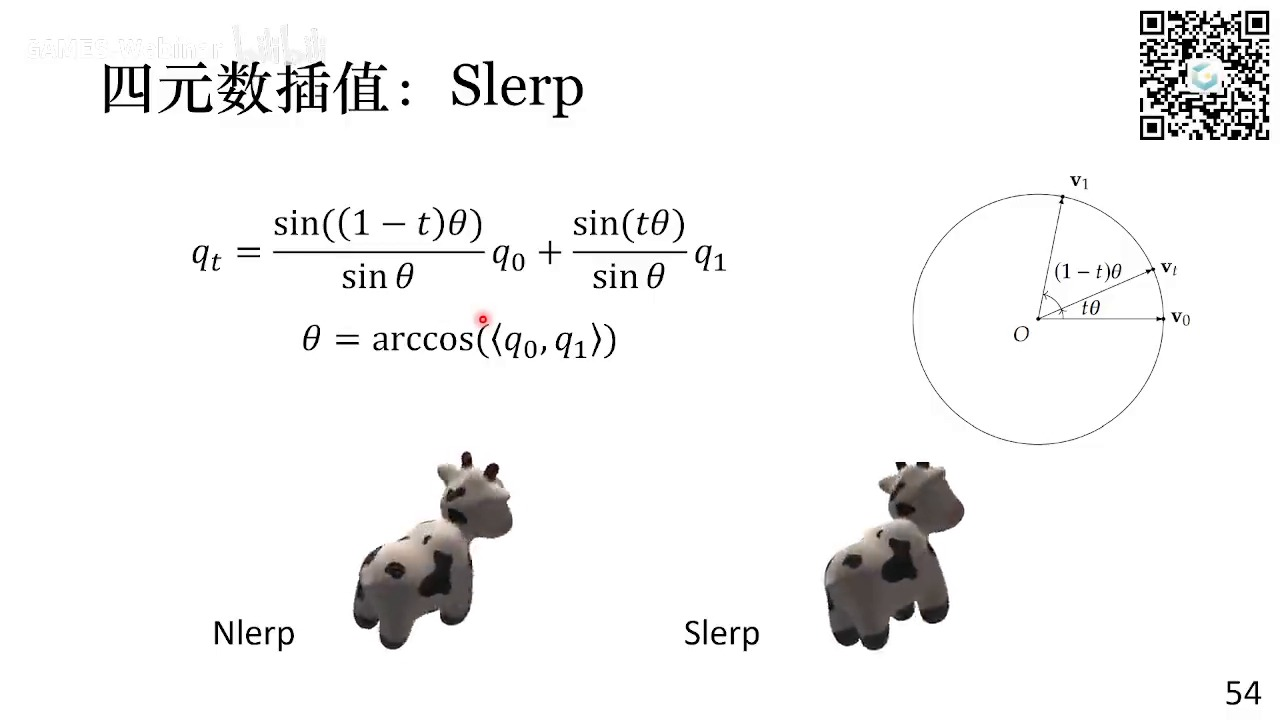
\includegraphics[width=0.92\textwidth]{figures/fig_39_slerp.jpg}
\caption{Slerp：沿大圆弧按角度等分，匀速旋转；与 Nlerp 的对比\vtag}
\end{figure}
\srcnote{01:33:45--01:34:00}
\end{minipage}


\begin{practicebox}{Slerp 的系数从哪里来}
在 $q_0,q_1$ 张成的平面内，设 $q_t=\alpha q_0+\beta q_1$。要求 $q_t$ 与 $q_0$ 的夹角为 $t\theta$，与 $q_1$ 的夹角为 $(1-t)\theta$，且 $\|q_t\|=1$。分别与 $q_0,q_1$ 做内积，得到 $\alpha+\beta\cos\theta=\cos t\theta$ 和 $\alpha\cos\theta+\beta=\cos(1-t)\theta$，解这个二元一次方程组，再用和差化积，就得到上面的 $\sin$ 系数。读者可以自己验证 $t=0$ 和 $t=1$ 时分别回到 $q_0$ 和 $q_1$。
\end{practicebox}

\subsection{最小弧}

由于 $q$ 与 $-q$ 表示同一个旋转，从 $q_0$ 到 $q_1$ 在球面上有两条路：一条是到 $q_1$ 的长弧，另一条是到 $-q_1$ 的短弧。二者的终点姿态相同，但长弧会朝着相差较大的方向绕远路，短弧走的距离更短，两个视频的对比非常明显。实现时，若 $\langle q_0,q_1\rangle<0$，应先把 $q_1$ 取反再插值。

\noindent\begin{minipage}{\textwidth}
\begin{figure}[H]
\centering
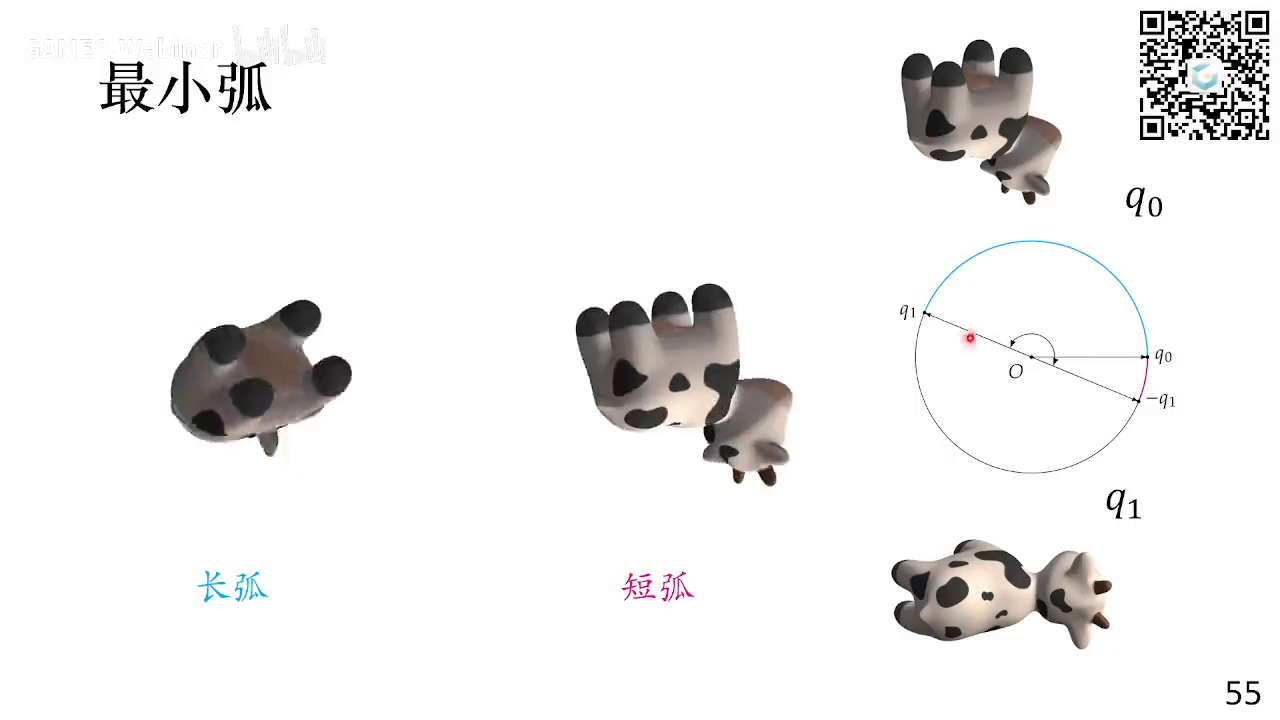
\includegraphics[width=0.92\textwidth]{figures/fig_40_shortest_arc.jpg}
\caption{最小弧：$q_1$ 与 $-q_1$ 对应同一旋转，应沿短弧插值\vtag}
\end{figure}
\srcnote{01:35:15--01:35:30}
\end{minipage}


\begin{warningbox}{插值前检查点乘符号}
四元数插值最常见的错误就是忘了处理双重覆盖。$\langle q_0,q_1\rangle<0$ 时，无论 Nlerp 还是 Slerp，都会走长弧，旋转多转了一大圈。此外，$\theta$ 很小时 $\sin\theta\approx0$，Slerp 的系数数值不稳定，通常退化为 Nlerp。
\end{warningbox}

\section{三种表示的比较与神经网络中的旋转}

\subsection{总结与比较}

\begin{itemize}
\item \textbf{欧拉角}：操作直观，但要注意规范（旋转顺序、内旋外旋），有万向锁，不好插值。
\item \textbf{轴角}：就是旋转的定义，但组合旋转需要转成矩阵运算，插值要用相对旋转。用于插值时效果不会特别好，因为直接插值走的不是最短路径。
\item \textbf{四元数}：计算效率高，方便组合，方便插值，方便采样；但理解不直观。最直观的理解方式反而是把四元数转换成轴角来看。

讲者补充了轴角插值与 Slerp 的关系：如果使用正确的相对旋转插值方法，轴角插值的结果与四元数 Slerp 是等价的，为什么等价也是作业的一部分。但实际中轴角插值用得比四元数少，因为它每一步都需要在矩阵和轴角之间来回转换，计算量大。至于直接对欧拉角做插值，可想而知效果不会特别好，因为它走的路径一般不是最短路径。
\end{itemize}

四元数之所以用得多，很大程度上是因为插值经常要用到。

\noindent\begin{minipage}{\textwidth}
\begin{figure}[H]
\centering
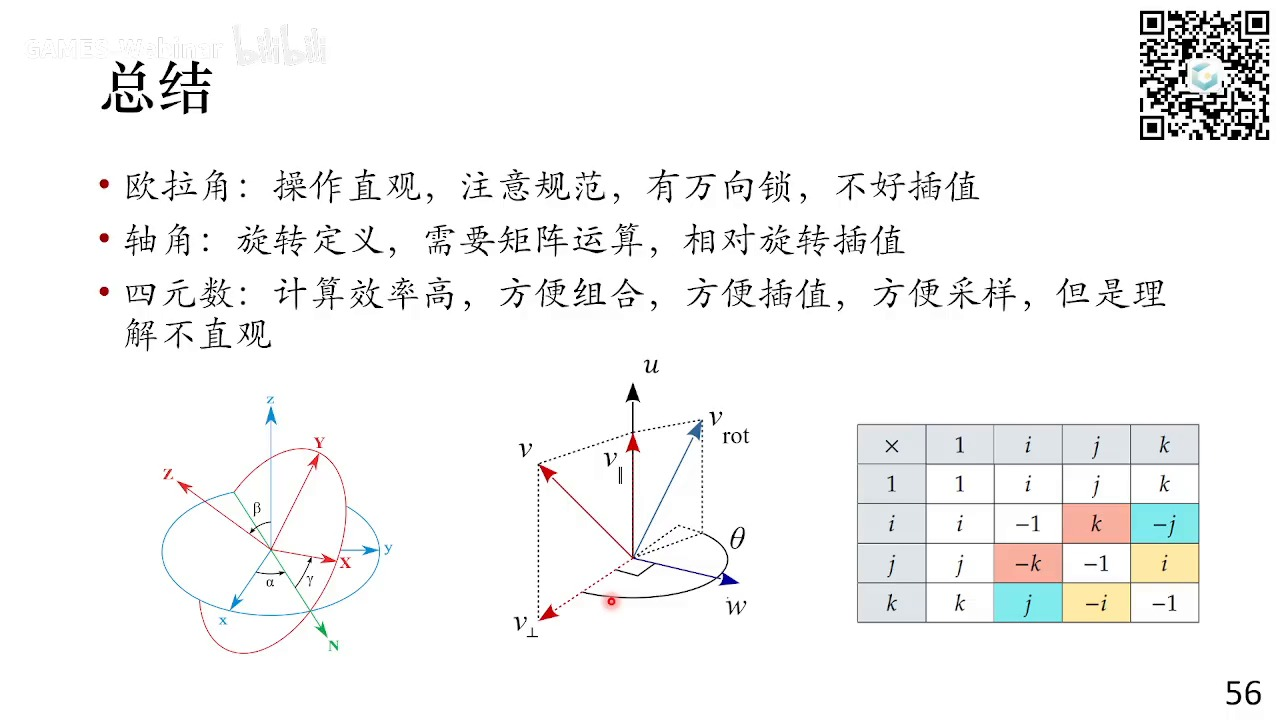
\includegraphics[width=0.92\textwidth]{figures/fig_41_summary_table.jpg}
\caption{三种旋转表示的总结：欧拉角、轴角、四元数\vtag}
\end{figure}
\srcnote{01:37:15--01:37:30}
\end{minipage}


\subsection{适合神经网络的旋转表示}

让神经网络输出旋转时，上面三种表示都有两个通病。

\textbf{多义性}。欧拉角中相差 $2\pi$ 的角度表示相同的旋转；轴角中 $(\mathbf v,\theta)$ 与 $(-\mathbf v,-\theta)$ 表示相同的旋转（课件写作 $(-\mathbf v,\pi-\theta)$；讲义作者注：按定义，绕 $-\mathbf v$ 转 $-\theta$ 或 $2\pi-\theta$ 才与绕 $\mathbf v$ 转 $\theta$ 相同）；四元数中 $q$ 与 $-q$ 结果相同。同一个旋转对应多个“正确答案”，会影响网络的优化。

\textbf{不连续}。若规定角度范围为 $[0,2\pi)$，那么在 $\theta=0$ 附近的相似旋转会被映射到区间的两个端点附近。讲者举例：原本 $+10^\circ$ 和 $-10^\circ$ 是相近的旋转，限制范围后变成 $10^\circ$ 和 $350^\circ$，相差很远。不连续的目标同样让网络难以学习。

\noindent\begin{minipage}{\textwidth}
\begin{figure}[H]
\centering
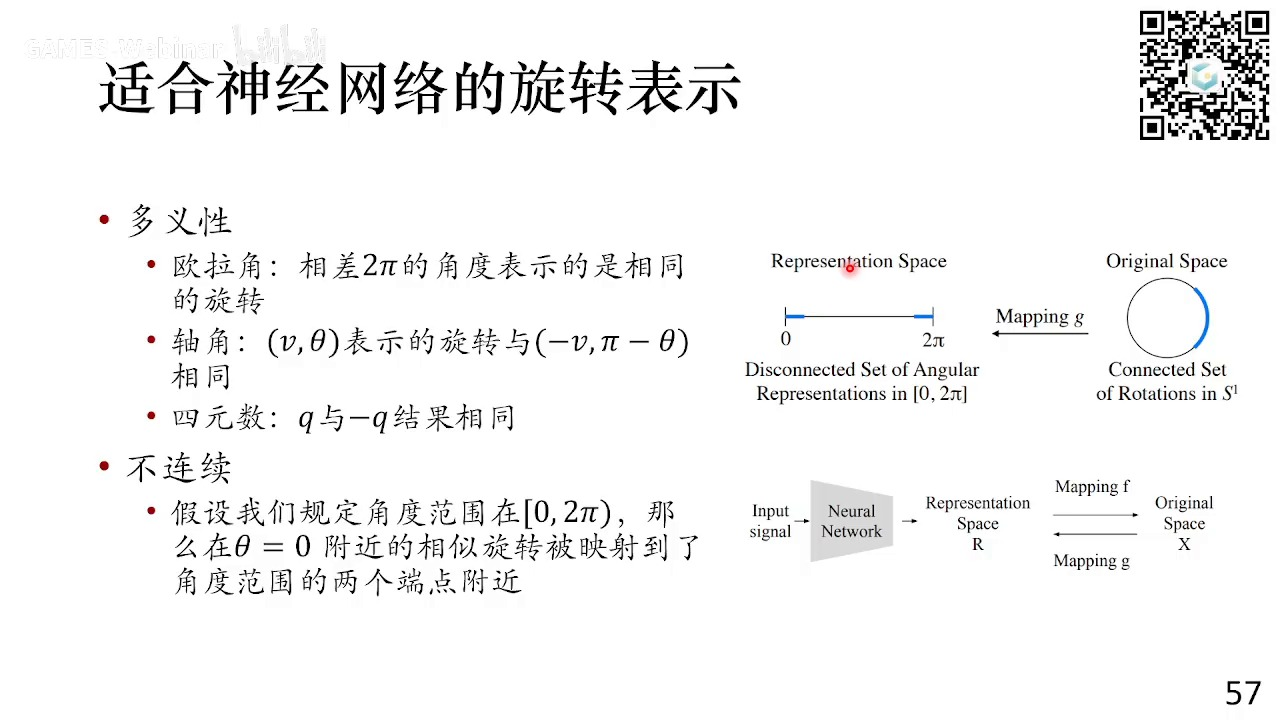
\includegraphics[width=0.92\textwidth]{figures/fig_42_nn_rep.jpg}
\caption{适合神经网络的旋转表示：多义性与不连续性\vtag}
\end{figure}
\srcnote{01:40:15--01:40:30}
\end{minipage}


\subsection{6D 旋转表示}

一个经典的方案是 6D 旋转表示。网络输出两个三维向量 $\mathbf a_1,\mathbf a_2$，再用 Gram–Schmidt 正交化构造旋转矩阵：
\[
\mathbf b_1=N(\mathbf a_1),\qquad
\mathbf b_2=N\big(\mathbf a_2-(\mathbf b_1\cdot\mathbf a_2)\mathbf b_1\big),\qquad
\mathbf b_3=\mathbf b_1\times\mathbf b_2,\qquad
\mathrm R=(\mathbf b_1,\mathbf b_2,\mathbf b_3),
\]
其中 $N(\cdot)$ 表示归一化。这样 $\mathbf b_1,\mathbf b_2,\mathbf b_3$ 都是单位向量且两两垂直，并且 $\mathbf b_3$ 由叉乘得到，保证 $\det\mathrm R=+1$，$\mathrm R$ 一定是旋转。6D 表示是冗余的，但它把一片连续的六维区域映射到旋转上，这种连续性正是网络喜欢的，所以在某些任务上它比四元数和轴角表现更好。

\noindent\begin{minipage}{\textwidth}
\begin{figure}[H]
\centering
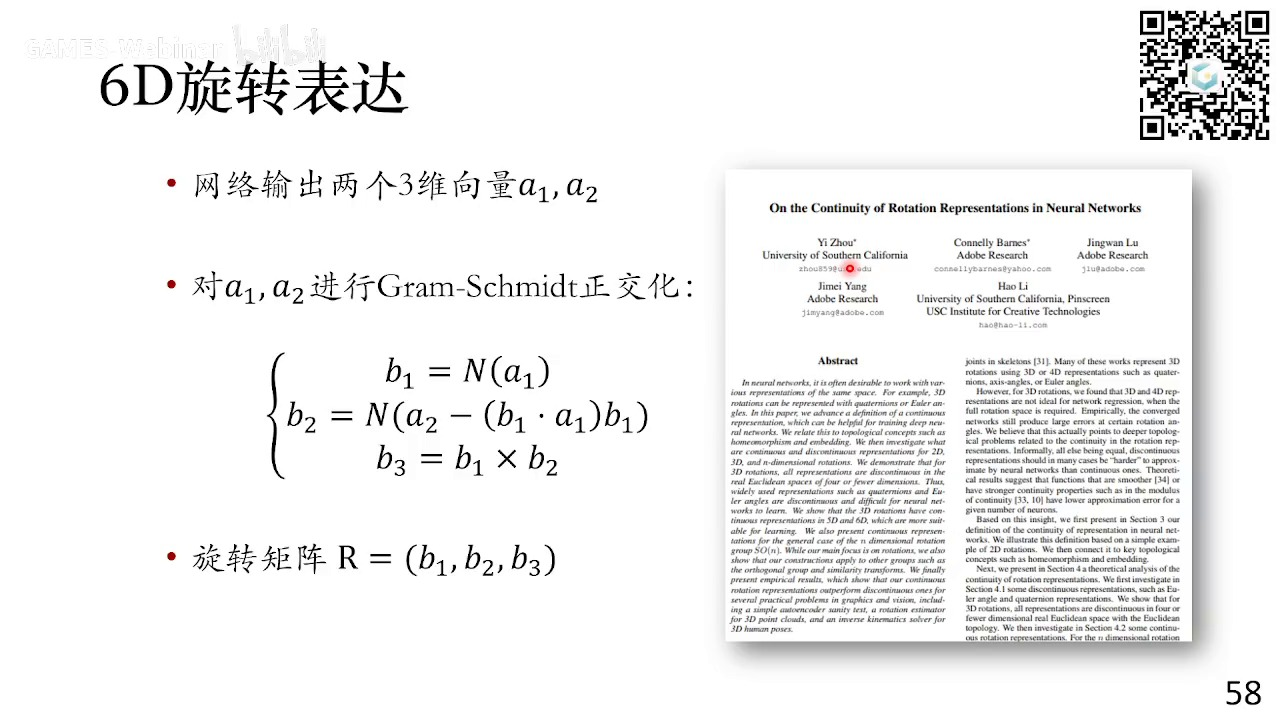
\includegraphics[width=0.92\textwidth]{figures/fig_43_sixd.jpg}
\caption{6D 旋转表示：两个三维向量经 Gram–Schmidt 正交化得到旋转矩阵\vtag}
\end{figure}
\srcnote{01:42:00--01:42:15}
\end{minipage}


\begin{warningbox}{课件中的一个小笔误}
课件的第二式写作 $N(\mathbf a_2-(\mathbf b_1\cdot\mathbf a_1)\mathbf b_1)$。讲者口头讲的是“从 $\mathbf a_2$ 中减去它在 $\mathbf b_1$ 上投影的部分”，所以应为 $\mathbf b_1\cdot\mathbf a_2$，上式已按此更正。
\end{warningbox}

不过，表示的好坏也不是绝对的，要根据具体任务选择。讲者举例，3D Gaussian Splatting 中每个高斯的朝向就用四元数表示；也有工作使用 9D 表示，直接输出 $3\times3$ 矩阵再投影到旋转，这样除了能建模旋转，还能建模旋转的不确定度。如果只是想直接拿来用，可以先试试 6D，一般效果还可以。

\noindent\begin{minipage}{\textwidth}
\begin{figure}[H]
\centering
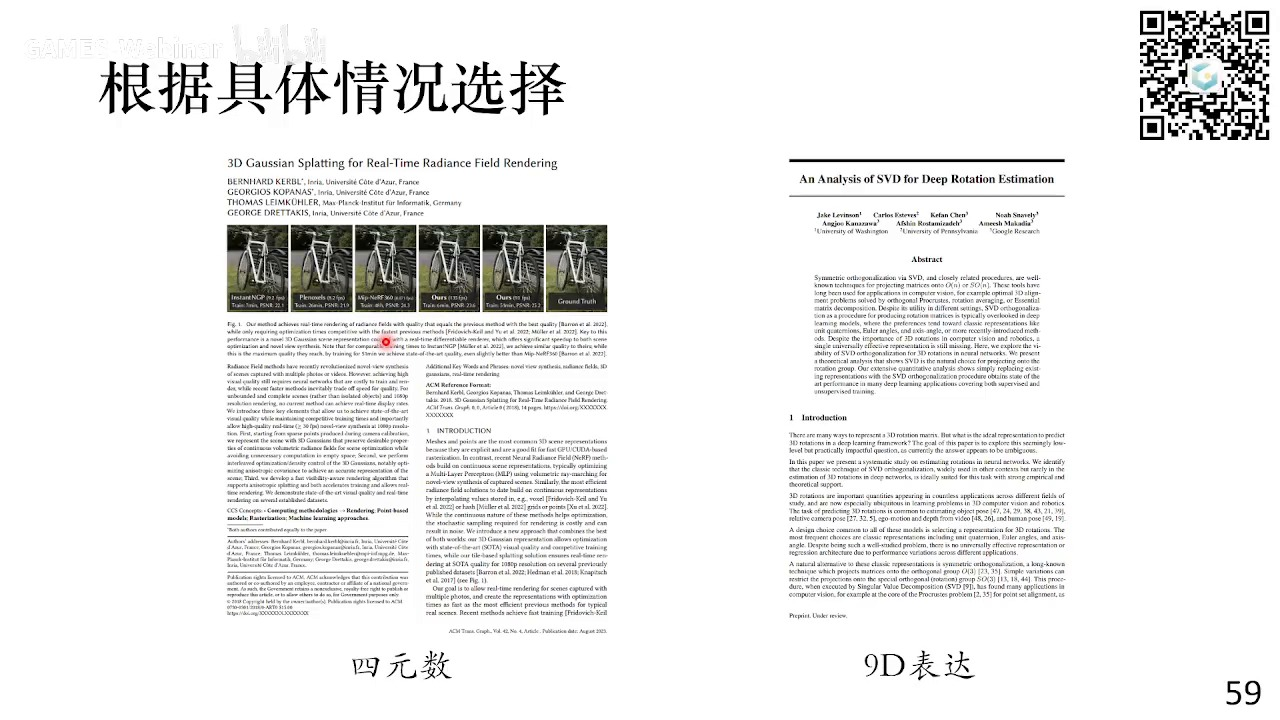
\includegraphics[width=0.92\textwidth]{figures/fig_44_choose_rep.jpg}
\caption{根据具体情况选择：四元数（如 3D Gaussian Splatting）与 9D 表示\vtag}
\end{figure}
\srcnote{01:43:00--01:43:15}
\end{minipage}


\section{角速度与旋转}

\subsection{角速度的定义}

最后一个问题是角速度与旋转的关系。做刚体模拟时，动力学方程都是用角速度或角动量建立的，所以必须知道角速度与旋转矩阵如何互相转换。

先从具体情况推。刚体上一点在局部坐标系下的坐标 $\mathbf x_l$ 是固定值，因为点随刚体一起转；世界坐标为 $\mathbf x_w=\mathrm R\mathbf x_l$。对时间求导，按物理定义，速度等于角速度叉乘位置：
\[
\dot{\mathbf x}_w=\boldsymbol\omega\times\mathbf x_w=[\boldsymbol\omega]\mathrm R\mathbf x_l ;\qquad
\dot{\mathbf x}_w=\dot{\mathrm R}\mathbf x_l+\mathrm R\dot{\mathbf x}_l=\dot{\mathrm R}\mathbf x_l .
\]
由于 $\mathbf x_l$ 任意，得到
\[
\dot{\mathrm R}=[\boldsymbol\omega]\mathrm R .
\]

另一个视角：旋转流形是 3 维的，角速度反映的应该是切空间中的量。对 $\mathrm R\mathrm R^{\mathsf T}=\mathrm I$ 求导，
\[
\dot{\mathrm R}\mathrm R^{\mathsf T}+\mathrm R\dot{\mathrm R}^{\mathsf T}=\dot{\mathrm R}\mathrm R^{\mathsf T}+(\dot{\mathrm R}\mathrm R^{\mathsf T})^{\mathsf T}=0,
\]
即 $\dot{\mathrm R}\mathrm R^{\mathsf T}$ 是反对称矩阵。任何 $3\times3$ 反对称矩阵都可以写成 $[\boldsymbol\omega]$ 的形式，所以 $[\boldsymbol\omega]=\dot{\mathrm R}\mathrm R^{\mathsf T}$ 也可以看成角速度的定义。讲者提醒，这里涉及对矩阵求导，可以回顾第二讲倪星宇讲的矩阵求导。这一推导的意义在于：$\dot{\mathrm R}$ 本身是 9 个数，但约束 $\mathrm R^{\mathsf T}\mathrm R=\mathrm I$ 对时间求导后告诉我们，$\dot{\mathrm R}$ 只能落在一个 3 维的子空间里，即旋转流形在 $\mathrm R$ 处的切空间，这 3 个数就是角速度。

\noindent\begin{minipage}{\textwidth}
\begin{figure}[H]
\centering
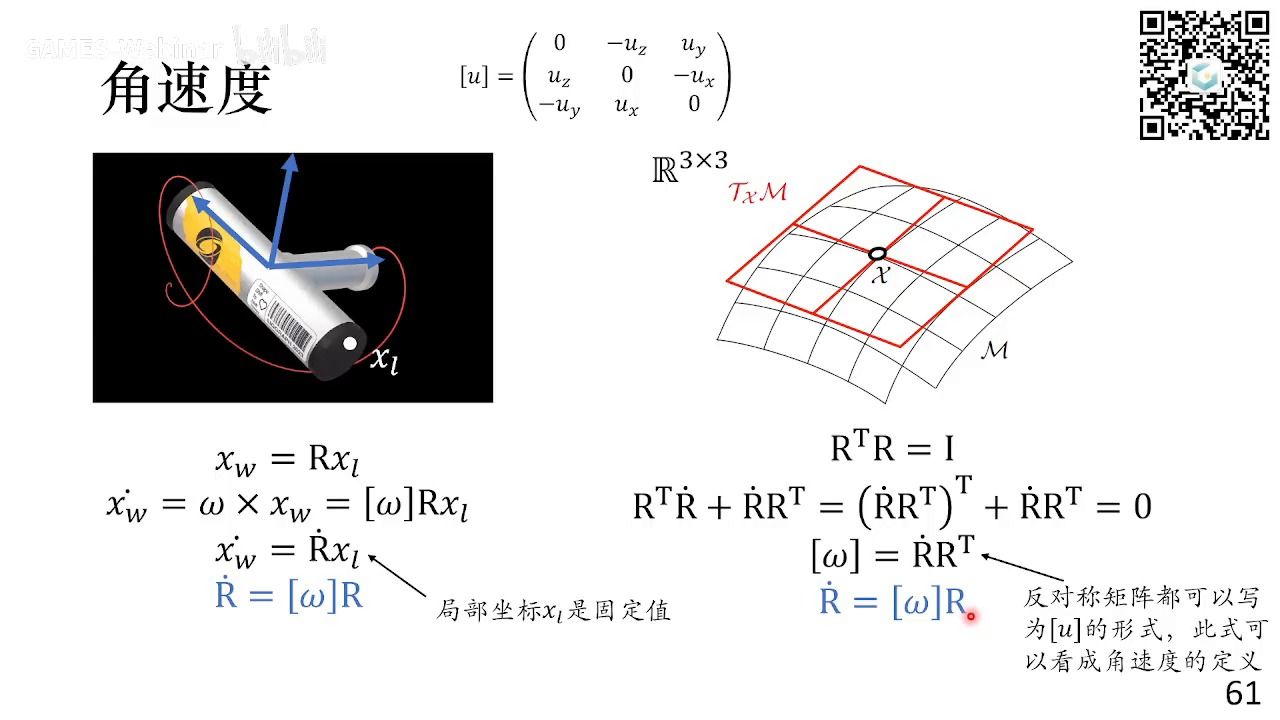
\includegraphics[width=0.92\textwidth]{figures/fig_45_angvel.jpg}
\caption{角速度：由 $\mathbf x_w=\mathrm R\mathbf x_l$ 求导得 $\dot{\mathrm R}=[\boldsymbol\omega]\mathrm R$，且 $\dot{\mathrm R}\mathrm R^{\mathsf T}$ 反对称\vtag}
\end{figure}
\srcnote{01:49:15--01:49:30}
\end{minipage}


\subsection{世界坐标角速度与局部坐标角速度}

上面的 $\boldsymbol\omega$ 是在世界坐标系下表达的。把 $[\boldsymbol\omega]\mathrm R$ 乘以任意向量 $\mathbf u$：
\[
[\boldsymbol\omega]\mathrm R\mathbf u=\boldsymbol\omega\times\mathrm R\mathbf u=\mathrm R\big((\mathrm R^{\mathsf T}\boldsymbol\omega)\times\mathbf u\big)=\mathrm R[\mathrm R^{\mathsf T}\boldsymbol\omega]\mathbf u ,
\]
这里用到旋转保持叉乘：$\mathrm R(\mathbf a\times\mathbf b)=(\mathrm R\mathbf a)\times(\mathrm R\mathbf b)$。由于 $\mathbf u$ 任意，
\[
\dot{\mathrm R}=[\boldsymbol\omega]\mathrm R=\mathrm R[\mathrm R^{\mathsf T}\boldsymbol\omega]=\mathrm R[\boldsymbol\omega'] ,\qquad \boldsymbol\omega'=\mathrm R^{\mathsf T}\boldsymbol\omega ,
\]
其中 $\boldsymbol\omega$ 是世界坐标角速度，$\boldsymbol\omega'$ 是局部坐标角速度。同一个旋转矩阵的导数，左乘用世界系角速度，右乘用局部系角速度。

\noindent\begin{minipage}{\textwidth}
\begin{figure}[H]
\centering
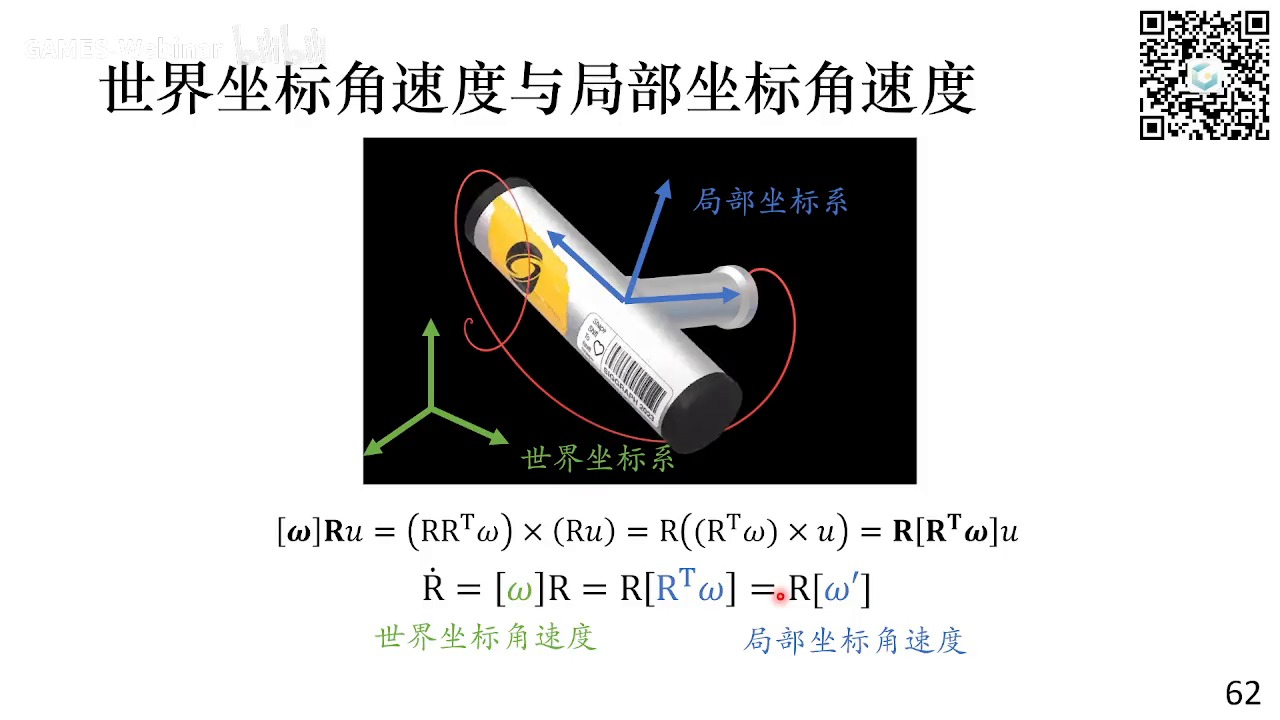
\includegraphics[width=0.92\textwidth]{figures/fig_46_world_local.jpg}
\caption{世界坐标角速度与局部坐标角速度：$\dot{\mathrm R}=[\boldsymbol\omega]\mathrm R=\mathrm R[\boldsymbol\omega']$\vtag}
\end{figure}
\srcnote{01:52:30--01:52:45}
\end{minipage}


\subsection{四元数与角速度}

用四元数也能推出类似的关系，推导稍繁琐。设 $\mathbf x_w=q\mathbf x_lq^*$，$\mathbf x_l$ 不变，所以
\[
\dot{\mathbf x}_w=\dot q\,\mathbf x_lq^*+q\mathbf x_l\,\dot q^*=(\dot qq^*)\,\mathbf x_w+\mathbf x_w\,(q\dot q^*) .
\]
这里用了 $\mathbf x_l=q^*\mathbf x_wq$。记 $s=\dot qq^*$。利用 $(pq)^*=q^*p^*$ 可知 $q\dot q^*=s^*$；对 $qq^*=1$ 求导又得 $s+s^*=0$，即 $s$ 是纯虚四元数，满足 $s^*=-s$。于是
\[
\dot{\mathbf x}_w=s\mathbf x_w-\mathbf x_ws=(0,\ 2\,\mathbf s\times\mathbf x_w),
\]
因为两个纯虚四元数相乘 $(0,\mathbf a)(0,\mathbf b)=(-\mathbf a\cdot\mathbf b,\ \mathbf a\times\mathbf b)$，交换次序时点乘部分相同、叉乘部分反号。另一方面 $\dot{\mathbf x}_w=\boldsymbol\omega\times\mathbf x_w$，对比得 $\boldsymbol\omega=2\mathbf s$，即 $\omega=2\dot qq^*$。整理并用 $\omega'=q^*\omega q$ 换到局部系，得到
\[
\dot q=\frac12\,\omega q=\frac12\,q\,\omega' ,
\]
其中 $\omega=(0,\boldsymbol\omega)$ 与 $\omega'=(0,\boldsymbol\omega')$ 分别是世界系和局部系的角速度写成的纯虚四元数。讲者说，对推导有兴趣的可以自己推一遍，没兴趣的直接记这个公式即可；做刚体模拟时，每一步就用它把角速度积分到四元数上，再归一化。

\noindent\begin{minipage}{\textwidth}
\begin{figure}[H]
\centering
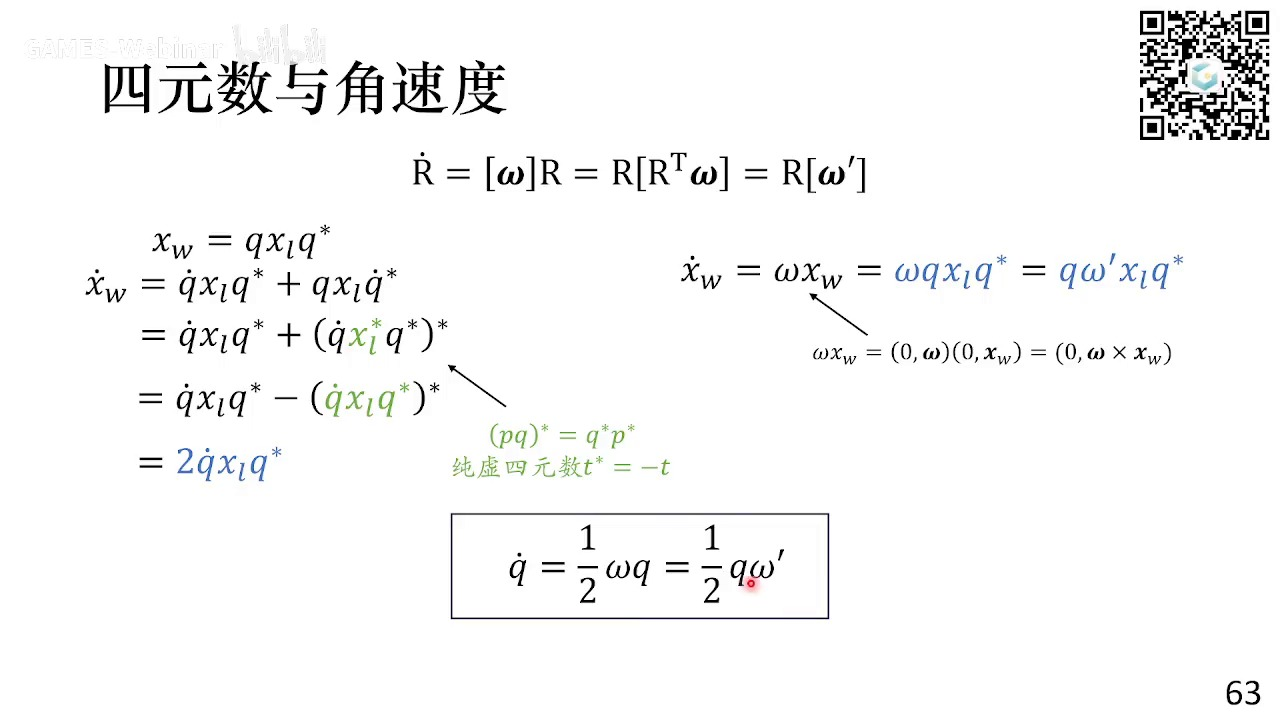
\includegraphics[width=0.92\textwidth]{figures/fig_47_quat_angvel.jpg}
\caption{四元数与角速度：$\dot q=\frac12\omega q=\frac12 q\omega'$\vtag}
\end{figure}
\srcnote{01:54:45--01:55:00}
\end{minipage}


\section{参考资料与自测}

讲者列出的参考资料有：Keenan Crane 的离散微分几何课程视频（B 站 BV1Pf4y1E7GJ），3Blue1Brown 的四元数视频（BV1SW411y7W1），Krasjet 的四元数讲义，刘利斌老师的角色动画课程（BV1GG4y1p7fF），Shinjiro Sueda 的刚体模拟代码 redmax，以及维基百科的相关词条。

\begin{practicebox}{自测清单}
\begin{itemize}
\item 从“刚体保持距离”推出 $\mathrm A^{\mathsf T}\mathrm A=\mathrm I$，并说明为什么还需要 $\det\mathrm R=1$。
\item 用约束计数说明二维旋转 1 个自由度、三维旋转 3 个自由度，并解释“9 维空间中的 3 维流形”。
\item 写出 $Z(\alpha)X(\beta)Z(\gamma)$ 的含义，说明万向锁出现在什么位置、损失了什么。
\item 推导罗德里格公式，并由 $\operatorname{tr}\mathrm R$ 和 $\mathrm R-\mathrm R^{\mathsf T}$ 反求轴角。
\item 用 Graßmann 积验证 $qvq^*$ 的实部为零，并说明为什么取半角。
\item 比较 Nlerp 与 Slerp，并说明为什么插值前要检查 $\langle q_0,q_1\rangle$ 的符号。
\item 写出 6D 表示的 Gram–Schmidt 构造，说明它为什么对神经网络更友好。
\item 推导 $\dot{\mathrm R}=[\boldsymbol\omega]\mathrm R=\mathrm R[\boldsymbol\omega']$。
\end{itemize}
\end{practicebox}

\end{document}
